\documentclass{article}
\usepackage[utf8]{inputenc}    
\usepackage[T1]{fontenc}       
\usepackage{lmodern}           
\usepackage{hyperref}
\hypersetup{
    colorlinks=true,       % false: boxed links; true: colored links
    linkcolor=blue,        % color of internal links (sections, etc.)
    urlcolor=cyan,         % color of external links
    linktoc=all            % 'all' makes both text and page number clickable
}
\usepackage{amsmath}   
\usepackage{algpseudocode}
\usepackage[ruled, vlined, algoruled]{algorithm2e} % Options for styling

\usepackage{amssymb}   
\usepackage{geometry}  
\usepackage{enumerate} 
\usepackage{xcolor}  
\usepackage{amsthm}
\usepackage{pdfpages}
\usepackage{mathrsfs}
\newtheorem{theorem}{Theorem}[section]
% \newtheorem{lemma}[theorem]{Lemma}
\newtheorem{corollary}[theorem]{Corollary}
% \newtheorem{definition}[theorem]{Definition}
\newtheorem{example}[theorem]{Example}
\usepackage{listings}  
\usepackage{tikz-cd}
\usetikzlibrary{positioning}
\usepackage{forest}     
\usepackage{xcolor}
\usepackage{tcolorbox}
\usepackage{stmaryrd}
\tcbuselibrary{theorems}

% remove/comment out the old line:
% \newtheorem{definition}[theorem]{Definition}

\usepackage{xcolor}
\usepackage{tcolorbox}
\tcbuselibrary{breakable}
\newtheorem{definition}[theorem]{Definition}
\let\olddefinition\definition
\let\endolddefinition\enddefinition
\renewenvironment{definition}
  {\begin{tcolorbox}[
      colback=red!10,
      colframe=red!50!black,
      boxrule=0.6pt,
      arc=2pt,
      left=6pt,right=6pt,top=4pt,bottom=4pt,
      breakable
    ]\olddefinition}
  {\endolddefinition\end{tcolorbox}}

\newtheorem{lemma}[theorem]{Lemma}
\let\oldlemma\lemma
\let\endoldlemma\endlemma
\renewenvironment{lemma}
  {\begin{tcolorbox}[
      colback=green!8,
      colframe=green!50!black,
      boxrule=0.6pt,
      arc=2pt,
      left=6pt,right=6pt,top=4pt,bottom=4pt
    ]\oldlemma}
  {\endoldlemma\end{tcolorbox}}

  \let\oldtheorem\theorem
\let\endoldtheorem\endtheorem
\renewenvironment{theorem}
  {\begin{tcolorbox}[
      colback=yellow!6,
      colframe=yellow!60!black,
      boxrule=0.6pt,
      arc=2pt,
      left=6pt,right=6pt,top=4pt,bottom=4pt,
      parbox=false
    ]\oldtheorem}
  {\endoldtheorem\end{tcolorbox}}
\usepackage{bussproofs}
\usetikzlibrary{arrows.meta}
\usetikzlibrary{arrows.meta,decorations.pathreplacing,calc}
\lstset{frame=tb,
  language=C,
  aboveskip=3mm,
  belowskip=3mm,
  showstringspaces=false,   
  columns=flexible,
  basicstyle={\small\ttfamily},
  numbers=none,
  numberstyle=\tiny\color{gray},
  keywordstyle=\color{blue},
  commentstyle=\color{brown},
  stringstyle=\color{orange},
  breaklines=true,
  breakatwhitespace=true,
  tabsize=3
}
\geometry{top=0.5in, bottom=0.5in, left=0.5in, right=1in}
% ctrl shift D to toggle night 
\begin{document}

\title{CS4269}
\author{Wang Xiyu A0282500R}
\date{}
\maketitle

\tableofcontents

\newpage
\section{Syntax of Propositional Logics}
\begin{definition}
    DSyntax decides what are allowed to be written
\end{definition}
\subsection{Well-formed Formula (WFF)}
A formula $\psi$ is obtained by composing $p \in P$ with $c\in C$, where $P$ is the set of propositions and $C$ is the set of connectors. here we use
any set of complete logic, like $C = \{\neg, \lor\}$. This is not a percise definition as counter examples that do not form 
a valid formula can be formulated based on this, for example $\neg \lor p$ means nothing. To formalize the definition we may attempt to define a language with the following grammar:
\[\Sigma = P\cup C\cup \{(, )\}\]
\[FORM :\{\psi = p \in P \mid \neg \psi \mid \psi \lor \psi \mid (\psi) \}\]
However this is a recursive definition as the definition of the a formula $\psi$ involves itself. We need to find a declarative way to define this recursive/inductive construction. 
\begin{definition}
    FORM is \textbf{the smallest} set of strings over $\Sigma$ where 
    \begin{enumerate}
        \item $P \subseteq FORM$
        \item $\forall \psi \in FORM, \neg \psi \in FORM$
        \item $\forall \psi_1, \psi_2 \in FORM, \psi_1 \lor \psi_2 \in FORM$
    \end{enumerate}
\end{definition}
We can see as a construction rule, we are admitting strings into the set of formula, but we need to somewhat impose restriction on what is not acceptable. 
\subsection{Closed Set}
Let's remove the attributive \textbf{the smallest} first and define another set that contains all the set that satisfy these rules listed above:
\begin{definition}
    Closed is a set of strings over $\Sigma$ where 
    \begin{enumerate}
        \item $P \subseteq Closed $
        \item $\forall \psi \in Closed, \neg \psi \in Closed$
        \item $\forall \psi_1, \psi_2 \in Closed, \psi_1 \lor \psi_2 \in Closed$
    \end{enumerate}
\end{definition}
\subsubsection{All Closed Set}
And we define a set ACS (All-closed sets). We can define FORM via the following constriction:
\[FORM = \bigcap ACS\]
Suppose $BCS = \emptyset$ and from definition
\[U_0 = \bigcap BCS = \{w \in \Sigma^* \mid \forall S \in BCS, w \in S\}\]
However, $BCS = \emptyset$, The statement $\forall S \in BCS, w \in S$ is vacuously true $\forall w \in \Sigma^*$, which means that
\[U_0 = \Sigma^* = \bigcap BCS\]
A contradiction.
Therefore we have proved that ACS cannot be empty, thus $\forall P, \exists S$ such that $S$ is a closed set. 
\subsection{FORM is the minimum of the set of Closed}
First let's prove that FORM is closed. It seems to be trivial that the intersection of closed sets is closed but formal proof is still needed.
We denote a set from the intersection construction as $T_0$.
\begin{lemma}
    $T_0$ is closed 
\end{lemma}
We are proving that the set $T_0$ we get from the intersection construction still satisfy the rules that define what is closed. 
\begin{proof}
    From rule 1,
    \begin{align*}
        \forall S &\in ACS, P \subseteq S\\
        &\rightarrow \forall p \in P, \forall S \in ACS, p \in S \\
        &\rightarrow \forall p \in P, p \in \bigcap ACS\\
        &\rightarrow P \in T_0
    \end{align*}
    From rule 2, 
    \begin{align*}
        \forall S &\in ACS, T_0 \subseteq S\\
        \text{let } w &\in T_0, \forall S \in ACS, w \in S, \neg w \in S\\
        & \rightarrow \forall w \in T_0, \neg w \in \bigcap ACS\\
        & \rightarrow \forall w \in T_0, \neg w \in T_0
    \end{align*}
    From rule 3,
    \begin{align*}
        \forall S&\in ACS, T_0 \subseteq S\\
        \text{let } w_1, w_2 &\in T_0, \forall S \in ACS, w_1 \lor w_2 \in S\\
        & \rightarrow \forall w_1, w_2 \in T_0, w_1 \lor w_2 \in \bigcap ACS\\
        & \rightarrow \forall w_1, w_2 \in T_0, w_1 \lor w_2 \in T_0
    \end{align*}
\end{proof}
\begin{lemma}
    $T_0$ is \textbf{a} smallest Closed set
\end{lemma}
\begin{proof}
    The proof of minimality is trivial. $T_0 = \bigcap ACS \rightarrow \forall S \in ACS, T_0 \subseteq S$
\end{proof}
\begin{lemma}
    $T_0$ is \textbf{the} smallest Closed set (unique). In other word, 
    \[\forall T_0' \in \{T \mid \forall S \in ACS, T \subseteq S\}, T_0' = T_0\]
\end{lemma}
Now we can use the generative rule to define formula, which is called \textbf{Backus-Naur form}. Note that a context-free grammar is a type of formal language. 
Backus Naur form is a specification language for this type of grammar. It is used to describe language syntax.
\subsection{Subformula}
\begin{definition}
$\phi_1$ is a subformula of $\phi_2$, denoted by 
\[\phi_1 \preccurlyeq \phi_2\]
as a relation is 
\begin{itemize}
    \item reflexive: $\forall \phi \in FORM, \phi \preccurlyeq \phi$
    \item transitive: $\forall \phi_1, \phi_2, \phi_3 \in FORM, (\phi_1 \preccurlyeq \phi_2) \land (\phi_2 \preccurlyeq \phi_3) \rightarrow \phi_1 \preccurlyeq \phi_3$
\end{itemize}  
Inductive definition:
\begin{align*}
    \forall \phi \in FORM, \phi \preccurlyeq (\neg \phi)\\
    \forall \phi_1, \phi_2 \in FORM, \phi_1 \preccurlyeq (\phi_1 \lor \phi_2)\\
    \phi_2 \preccurlyeq (\phi_1 \lor \phi_2)
\end{align*}
\end{definition}
We might intuitively think that subformula can be defined using the notion of substring, since we have been considering formula as concatenation of 
proposition and connector symbols. However based on out inductive definition, we can come up with the following counter example to a definition using substring: 
A formula $\phi_1$ is a subformula of $\phi_2$ if and only if $\phi_1$ is a well-formed formula, and is a substring to $\phi_2$
\[p \lor q \not\preccurlyeq \neg p \lor q\]
\textcolor{red}{What if we tighten the syntax by strictly enforce the use of parenthese whenver we can}

\section{Sematics of Propositional Logics}
\begin{definition}
    Sematics describe meanings.
\end{definition}
\subsection{Truth Assignment/Proposition evaluation}
A truth assignment or a valuation of propositions is a function that maps from the set of propositions to true and false.
\[v: P \rightarrow \{T, F\}\]
\[v \in [P \rightarrow \{T, F\}]\]
\begin{example}
    Consider $v = \{p_1 \mapsto T, p_2 \mapsto F\}$, we can derive
    \begin{align*}
    v&(p_1) = T\\
    v&(p_2)= F\\
    v&(\neg p_2) = T\\
    v&(p_1\lor p_2) = T \text{ etc.}
    \end{align*}
\end{example}
\subsection{Entail/Model}
We denote entailment of an evaluation function to formula as 
\[v \models \psi\]
We also indeuctively define the following rule 
\begin{align*}
    \forall p \in P, v\models p &\iff v(p)\\
     v\models \psi &\iff v\nvDash \neg \psi\\
     v \models \psi_1 \lor \psi_2 &\iff (v\models \psi_1) \lor (v\models \psi_2)
\end{align*}
\subsubsection{Valuation and Model}
A valuation $v$ is a model of a formula $\phi$, if and only if $v(\phi) = T$. 
\begin{itemize}
    \item $\forall \phi \text{ over } P, \exists 2^{|P|}$ valuations.
    \item A formula can have many or one or none models 
\end{itemize}

\subsubsection{$\models$ as a relation}
\begin{definition}
    $\models \text{ } \subseteq \{2^{|P|} \times FORM\}$ is a binary relation, between truth assignment to formula. 
    We define as follows: 
    \begin{itemize}
        \item $\forall p \in P, v \models p \iff v(p) = 1$
        \item $v \not\models p$ otherwise.
    \end{itemize}
    Consider a valuation $v$ as a subset of $P$ such that the propositions in $v$ denoted by $v(p)$ is assigned with true. $v \in \mathscr{P}(P)$
\end{definition}
$$
\begin{array}{|c|c||c|c|c|c|c|}
\hline
\phi & \psi & \neg \phi & (\phi \wedge \psi) & (\phi \vee \psi) & (\phi \to \psi) & (\phi \leftrightarrow \psi) \\
\hline
0 & 0 & 1 & 0 & 0 & 1 & 1 \\
\hline
0 & 1 & 1 & 0 & 1 & 1 & 0 \\
\hline
1 & 0 & 0 & 0 & 1 & 0 & 0 \\
\hline
1 & 1 & 0 & 1 & 1 & 1 & 1 \\
\hline
\end{array}
$$
\begin{definition}
    \[p(v) = v(p)\]
    A proposition can be viewed as a circuit is jsut a wire, thus if a proposition is assigned with true by a valuation, the valuation valuates this proposion to be true
\end{definition}
\begin{lemma}
    Let $\phi \in FORM, v \in \mathscr{P}(P), v \models \phi \iff \phi(v) = 1$
\end{lemma}
\begin{proof}
    Base case: $\forall \phi = p \in P, v\models \phi \iff v(p) = 1 \iff p(v) = 1$\\
    Inductive case: 
    \begin{enumerate}
        \item 
    \end{enumerate}
\end{proof}
\subsubsection{Logical Equivalence}
\begin{definition}
    Syntax definition of logical equivalence is as follows: 
    \[\phi_1 \equiv \phi_2 \iff \forall v: P \mapsto \{T, F\} (v\models \phi_1),  v \models \phi_2\]
\end{definition}
\begin{example}
    \[p \lor (\neg p) \equiv q \lor (\neg q)\]

\begin{align*}
    &\forall v \models (p \lor (\neg p)), \\
    &v \models p \text{ or } v \models (\neg p)\\
    &v \models p \text{ or } v \not\models p\\
    &\forall v: P \mapsto \{T, F\}, 
\end{align*}
\textcolor{red}{TODO}
\end{example}
\subsection{Satisfiability of Formula}
\begin{definition}
    Let $\phi \in FORM, \phi $ is satisfiable 
    \[\iff \exists v: P \mapsto \{T, F\}, v \models \phi\]
\end{definition}
\subsubsection{Valid formula(tautology)}
\begin{definition}
    Tautology: $\phi$ is a tautology $\iff \forall v, v \models \phi$
\end{definition}
\begin{example}
    \[\phi = \neg(p \lor (\neg p))\]
    From example 2.4, we have 
    \begin{align*}
        &\forall v, v \models (p \lor (\neg p))\\
        &\rightarrow \forall v, v \not\models \neg(p \lor (\neg p))
    \end{align*}
    Thus $\phi$ is NOT satisfiable.
\end{example}

\subsection{Satisfiability of a set of formula}
\subsubsection*{Set Satisfication}
\begin{definition}
    Let $\Gamma \subseteq FORM$, 
    \[v \models \Gamma \iff \forall \phi \in \Gamma, v \models \phi\]
\end{definition}
\subsubsection*{Set Satisfiability}
\begin{definition}
        Let $\Gamma \subseteq FORM$, $\Gamma$ is satisfiable 
    \[\iff \exists v, \forall \phi \in \Gamma, v \models \phi\]
\end{definition}
\begin{example}
     $\Gamma = \emptyset$, $\Gamma$ is satisfiable.
    \begin{proof}
        Consider $v: P \mapsto \{T, F\}, v(p) = T \forall p \in P$, 
        $\forall \phi \in \Gamma, v \models \phi$ is vacuously true.
    \end{proof}
\end{example}
\begin{example}
     $\Gamma = FORM$, $\Gamma$ is NOT satisfiable.
     \begin{proof}
        Suppose otherwise,
        \begin{align*}
            \exists v, \forall \phi &\in \Gamma, v \models \phi\\
            \forall \phi &\in \Gamma, (\neg \phi) \in \Gamma\\
            &v \models (\neg \phi)
        \end{align*}
        A contradiction.
     \end{proof}
\end{example}
\subsubsection{Relevance}
\begin{definition}
    Define set $OCCUR(\phi) \subseteq P$, which contains propositions appear in $\phi$. Inductively defined as
    \begin{align*}
        &OCCUR(\phi) = \{p\} \iff \phi \equiv p,p \in P\\
        &OCCUR(\neg \phi) = OCCUR(\phi)\\
        &OCCUR(\phi_1 \lor \phi_2) = OCCUR(\phi_1) \cup OCCUR(\phi_2)
    \end{align*} 
\end{definition}
\begin{lemma}
    Let $\phi \in FORM$, let $v_1, v_2$ be valuations over $P$. 
    \[\forall p \in OCCUR(\phi), v_1(p) = v_2(p) \rightarrow (v_1 \models \phi \rightarrow v_2 \models \phi)\]
    $v_1, v_2$ can be different valuations over $p' \notin OCCUR(\phi)$
\end{lemma}
\begin{proof}
Let $p \in P, $
\end{proof}
\subsubsection{Logical consequence}
Semantic logical consequence:
\begin{definition}
    \[\Gamma \models \phi \iff \forall v \models \Gamma, v \models \phi\]
\end{definition}
\noindent Syntactic logical consequence: (logical deriability)
\begin{definition}
    A formula $\phi$ is a syntactic consequence of $\Gamma$ 
    if there exists a formal proof (a finite sequence of formulas) ending in $\phi$, where each step is either a premise from $\Gamma$, an axiom, or follows from previous steps via an inference rule (like Modus Ponens).
\end{definition}
\noindent \textbf{Material Implication $(\rightarrow)$ vs. Logical Consequence $(\models)$}
\begin{itemize}
    \item Material implication is a connector within a formula, $p \rightarrow q \equiv \neg(p \lor q)$, and can therefore be eval to true or false in a single model.
    \item Logical consequence is a relation between formulas (meta-logic), it is a statement about all models. $\{p, p\rightarrow q\}\models q$
\end{itemize}
\subsection{Modelling Computations as Propositional Logic}
Computation problems can be considered as membership check of an encoded problem instance to a language. 
\[L = \{p \mid \langle M, p\rangle\}\]
Here instead of arbituary encoding, we consider problem encoding with propositional logics only, 
and solve with SAT solvers by deciding whether the set of formula we form from any instance of the problem is satisfiable.
That is 
\[Encode: p \mapsto FORM, \forall p, \exists v \models Encode(p) \iff p \in L\]
The rules of such modelling include:
\begin{itemize}
    \item Propositional logics only
    \item The final expression must one well formed fomula
    \item for problem of size $n$, the size of the formula $\phi$ must be in $O(poly(n))$
\end{itemize}
Note that there can be different definition on the size of the 
\begin{itemize}
    \item problem: in unary, binary etc; 
    \item Formula: Whether by the number of nodes in the syntax tree or length of the string \textcolor{red}{Anything else?}
\end{itemize}

\begin{example}
    Graph coloring problem: given a undirected graph $G = (V, E)$, whether there exists a $k$ coloring of all vertices such that no neighbouring vertices have the same color.\\
    Consider the following construction of a proposition set $P$:
    \[P = \{p_{v, i} \mid v \in V, i \in [1, k]\}\]
    The valuation of proposition $p_{v, i}$ conceptually represents vertex $v$ is assigned color $i$. \\
    We can formulate constriants as well formed formula, and use conjunction to connect the formula to model satisfaction of multiple constraints. 
    \begin{corollary}
        $\forall \phi_1, \phi_2 \in FORM, (\phi_1 \land \pi_2) \in FORM$
    \end{corollary}
    First let us list down the constraints of this problems, including implicit ones in plain words
    \begin{enumerate}
        \item Neighbouring vertices have different colors.
        \item All vertices as assigned with exactly one color.
    \end{enumerate}
    \subsubsection*{1. $\phi_{nbr}$}
    First lets formula the constraint between any 2 vertices, 
    \[\forall (\alpha, \beta) \in E, c(v_\alpha) \neq c(v_\beta)\]
    And from our proposition set, $c(v_\gamma) = i \iff \exists v, v\models p_{\gamma, i}$. As such we have 
    \[\phi_{\alpha, \beta, i} = \neg(p_{\alpha, i} \land p_{\beta, i})\]
    This models vertex $\alpha$ and vertex $\beta$ are not colored with color $i$ at the same time.
    For every color this needs to hold, thus we have 
    \[\phi_{nbr(\alpha, \beta)} = \bigwedge_{i \in [1, k]} \phi_{\alpha, \beta, i}\]
    For every pair of neighbouring vertices this also needs to hold. Therefore we have 
    \[\phi_{nbr} = \bigwedge_{(\alpha, \beta) \in E}\phi_{nbr(\alpha, \beta)}\]
    \subsubsection*{2. $\phi_{exactly-1}$}
    To model exactly 1 coloring on each vertex, we can formulate $\phi_{\geq 1}$ and $\phi_{\leq 1}$ first and use conjunction to connect them.
    Given our propositions, to make sure vertex $v$ is at least assign a color ($\phi_{v, \geq 1}$), 
    \[\phi_{v, \geq 1} = \bigvee_{i \in [1, k]} p_{v, i}\]
    This needs to hold for every vertex, thus we have 
    \[\phi_{\geq 1} = \bigwedge_{v \in V} \phi_{v, \geq 1}\]
    Then we need to model at most 1, (or less than 2) coloring on each vertex. Vertex $v$ is not assignment with both color $i$ and $j$ can be formulated as 
    \[\phi_{v, i, j,\leq 1} = \neg(p_{v, i} \land p_{v, j})\]
    This needs to hold for every distinct pair of colors, thus
    \[\phi_{v, \leq 1} = \bigwedge_{i \neq j \in [1, k]} \phi_{v, i, j, \leq 1}\]
    For all vertices
    \[\phi_{\leq 1} = \bigwedge_{v\in V} \phi_{v, \leq 1}\]
    Finally we have 
    \[\phi_{exactly-1} = \phi_{\leq 1} \land \phi_{\geq 1}\]
    And the overall formula for an instance of $G = (V, E)$ becomes 
    \[\phi = \phi_{nbr} \land \phi_{exactly-1}\]
\end{example}
Similar to reduction, we need also now to show that 
\[\exists v: P \mapsto \{T, F\}, v \models \phi \iff \langle G = (V, E), k\rangle \in L_{color}\]
\textcolor{red}{TODO}

\begin{center}
\emph{Introduce propositional variables that encode atomic choices, then add
constraints that enforce the combinatorial structure of the problem.}
\end{center}

\subsubsection*{1. Hamiltonian Path}

\paragraph{Instance.}
Graph $G=(V,E)$ with $|V|=n$.

\paragraph{Variables.}
For every vertex $v \in V$ and position $i \in \{1,\dots,n\}$:
\[
X_{v,i} \quad \text{``vertex $v$ is at position $i$ in the path.''}
\]

\paragraph{Constraints.}

\begin{enumerate}
    \item \textbf{Each position has exactly one vertex:}
    \[
    \bigvee_{v \in V} X_{v,i}
    \quad\text{and pairwise exclusion.}
    \]
    \item \textbf{Each vertex appears exactly once:}
    \[
    \bigvee_{i=1}^{n} X_{v,i}
    \quad\text{and pairwise exclusion.}
    \]
    \item \textbf{Adjacency constraint:}
    If $(u,v) \notin E$, then for all $i$:
    \[
    \neg X_{u,i} \lor \neg X_{v,i+1}.
    \]
\end{enumerate}

Satisfiable iff $G$ has a Hamiltonian path.

\bigskip

\subsubsection*{2. Clique of Size $k$}

\paragraph{Instance.}
Graph $G=(V,E)$.

\paragraph{Variables.}
For each vertex $v \in V$:
\[
X_v \quad \text{``vertex $v$ is selected.''}
\]

\paragraph{Constraints.}

\begin{enumerate}
    \item \textbf{At least $k$ vertices selected:}
    Encode using a cardinality constraint.
    \item \textbf{Selected vertices form a clique:}
    If $(u,v) \notin E$, then
    \[
    \neg X_u \lor \neg X_v.
    \]
\end{enumerate}

Satisfiable iff there exists a clique of size $\ge k$.

\bigskip

\subsubsection*{3. 3-Dimensional Matching}

\paragraph{Instance.}
Sets $X,Y,Z$ and triples $T \subseteq X \times Y \times Z$.

\paragraph{Variables.}
For each triple $t \in T$:
\[
X_t \quad \text{``triple $t$ is chosen.''}
\]

\paragraph{Constraints.}

\begin{enumerate}
    \item \textbf{No element used twice:}

    If triples $t,t'$ share an element, then
    \[
    \neg X_t \lor \neg X_{t'}.
    \]

    \item \textbf{Select exactly $k$ triples:}
    Encode cardinality constraint.
\end{enumerate}

Satisfiable iff there is a matching of size $k$.

\bigskip

\subsubsection*{4. Subset Sum}

\paragraph{Instance.}
Numbers $a_1,\dots,a_n$, target $B$.

\paragraph{Variables.}
\[
X_i \quad \text{``$a_i$ is selected.''}
\]

\paragraph{Constraints.}

We encode:
\[
\sum_{i=1}^n a_i X_i = B.
\]

This is reduced to propositional logic by building a binary addition circuit:

\begin{itemize}
    \item Introduce variables for each bit of partial sums.
    \item Encode full-adder constraints using propositional clauses.
\end{itemize}

Satisfiable iff there exists a subset summing to $B$.

\bigskip

\subsubsection*{5. Exact Cover}

\paragraph{Instance.}
Universe $U$, collection $\mathcal{S} = \{S_1,\dots,S_m\}$.

\paragraph{Variables.}
\[
X_i \quad \text{``set $S_i$ is selected.''}
\]

\paragraph{Constraints.}

For every element $u \in U$:

\begin{enumerate}
    \item \textbf{At least one covering set:}
    \[
    \bigvee_{u \in S_i} X_i
    \]
    \item \textbf{At most one covering set:}
    If $u \in S_i \cap S_j$ and $i \neq j$:
    \[
    \neg X_i \lor \neg X_j.
    \]
\end{enumerate}

Satisfiable iff an exact cover exists.

\bigskip

\subsubsection*{6. Scheduling with Precedence Constraints}

\paragraph{Instance.}
Tasks $T_1,\dots,T_n$, time slots $1,\dots,m$.

\paragraph{Variables.}
\[
X_{i,t} \quad \text{``task $i$ scheduled at time $t$.''}
\]

\paragraph{Constraints.}

\begin{enumerate}
    \item Each task scheduled exactly once.
    \item At most one task per time slot.
    \item If $T_i$ must precede $T_j$:
    \[
    X_{i,t} \rightarrow
    \bigvee_{t' > t} X_{j,t'}.
    \]
\end{enumerate}

\bigskip
\subsection{Encoding a Full Adder in Pure Propositional Logic}

A full adder takes three input bits:

\[
x,\; y,\; c_{in}
\]

and produces two outputs:

\[
s \quad (\text{sum bit}), \qquad c_{out} \quad (\text{carry bit})
\]

Semantically:

\[
s = x \oplus y \oplus c_{in}
\]
\[
c_{out} = (x \land y) \lor (x \land c_{in}) \lor (y \land c_{in})
\]

We now encode this purely in propositional logic using only
$\land,\lor,\neg$ (or $\to,\bot$ if preferred).

\bigskip
\subsubsection*{1. Encoding the Sum Bit}

The sum is true iff an odd number of inputs are true.

Truth table characterization:

\[
s \leftrightarrow
(x \land \neg y \land \neg c_{in})
\lor
(\neg x \land y \land \neg c_{in})
\lor
(\neg x \land \neg y \land c_{in})
\lor
(x \land y \land c_{in})
\]

Thus we encode:

\[
(s \rightarrow \Phi_s)
\;\land\;
(\Phi_s \rightarrow s)
\]

where $\Phi_s$ is the disjunction above.

\bigskip
\subsubsection*{2. Encoding the Carry Bit}

Carry is true iff at least two inputs are true:

\[
c_{out} \leftrightarrow
(x \land y)
\lor
(x \land c_{in})
\lor
(y \land c_{in})
\]

Again encode as:

\[
(c_{out} \rightarrow \Phi_c)
\;\land\;
(\Phi_c \rightarrow c_{out})
\]

\bigskip
\subsubsection*{3. CNF Encoding (SAT-friendly)}

To encode for SAT, we introduce clauses.

\paragraph{Carry Constraints}

\[
\neg c_{out} \lor x \lor y
\]
\[
\neg c_{out} \lor x \lor c_{in}
\]
\[
\neg c_{out} \lor y \lor c_{in}
\]

\[
\neg x \lor \neg y \lor c_{out}
\]
\[
\neg x \lor \neg c_{in} \lor c_{out}
\]
\[
\neg y \lor \neg c_{in} \lor c_{out}
\]

\bigskip
\paragraph{Sum Constraints (XOR Form)}

We can encode $s = x \oplus y \oplus c_{in}$ using clauses:

\[
(x \lor y \lor c_{in} \lor \neg s)
\]
\[
(\neg x \lor \neg y \lor c_{in} \lor \neg s)
\]
\[
(\neg x \lor y \lor \neg c_{in} \lor \neg s)
\]
\[
(x \lor \neg y \lor \neg c_{in} \lor \neg s)
\]

\[
(\neg x \lor \neg y \lor \neg c_{in} \lor s)
\]
\[
(x \lor y \lor \neg c_{in} \lor s)
\]
\[
(x \lor \neg y \lor c_{in} \lor s)
\]
\[
(\neg x \lor y \lor c_{in} \lor s)
\]

These clauses exactly encode the XOR behavior.

\bigskip
\subsubsection*{4. Circuit-Style Encoding (Cleaner)}

Instead of expanding XOR directly, introduce auxiliary variables:

\[
t = x \oplus y
\]
\[
s = t \oplus c_{in}
\]

Each XOR can be encoded with 4 clauses:

\[
(t \leftrightarrow x \oplus y)
\]

which in CNF becomes:

\[
(\neg x \lor \neg y \lor \neg t)
\land
(x \lor y \lor \neg t)
\land
(x \lor \neg y \lor t)
\land
(\neg x \lor y \lor t)
\]

This keeps formula size linear.

\bigskip
\subsubsection*{5. Why This Matters}

Full adders are the atomic building blocks of:

\begin{itemize}
    \item Binary addition circuits
    \item Subset Sum encodings
    \item Integer programming to SAT reductions
    \item Cook--Levin tableau arithmetic
\end{itemize}

Any arithmetic constraint can be reduced to propositional logic
by composing full adders.

\bigskip
\subsubsection*{Conceptual Insight}

Arithmetic $\longrightarrow$ Circuits $\longrightarrow$ Propositional Logic

This translation is what makes SAT complete for NP:
even numeric computation can be flattened into Boolean structure.
\subsubsection*{General Pattern}

Almost all NP problems can be modelled by:

\begin{enumerate}
    \item Encoding choices with propositional variables.
    \item Enforcing structural constraints with local clauses.
    \item Encoding counting via cardinality circuits if needed.
\end{enumerate}

This modelling perspective is precisely what makes SAT solvers
universal engines for combinatorial search.

\section{Compactness Theorem for Propositional Logics}
\begin{definition}
    Axiom of Choice: formally
    \[\forall X, \emptyset \in X \lor \exists f, dom(f)= X \land \forall A \in X, f(A) \in A\]
    A choice function (or selection) $f$ defined on a collection of nonempty sets $X$, such that for every set $A$ in the collection $X$,
    $f(A)$ is an element in $A$. That is, Axiom—For any set $X$ of nonempty sets, 
    there exists a choice function $f$ that is defined on $X$ and maps each set of $X$ to an element of that set. 
\end{definition}
\begin{theorem}
    If $P$ is finite, $FORM$ over $P$ is finite.
\end{theorem}
\begin{theorem}
    If $P$ is countable, $FORM$ over $P$ is countable.
\end{theorem}
\begin{proof}
    Given $\forall \phi \in FORM, \phi$ is finitely long, this theorem is another way of stating: The language formed from countable 
    alphabet $P\cup C$ with the inductive construction rules, is countable. We can prove a stronger theorem first. 
\end{proof}
\begin{theorem}
    All languages formed from a countable alphabet is countable. 
\end{theorem}
\begin{proof}
    Consider $L = \Sigma^*$, we will prove that $\Sigma$ is countable $\rightarrow L$ is countable. We use the same diagnol proof for the countability of $\mathbb{Q}$ to show an enumaration of all strings 
    formable from a countable alphabet.
\usetikzlibrary{arrows.meta}
\begin{figure}[h]
    \centering
    % --- Left Minipage: Rationals ---
    \begin{minipage}[t]{0.48\textwidth}
        \centering
        \textbf{Rational Numbers ($\mathbb{Q}^+$)}
        \vspace{0.5cm}
        
        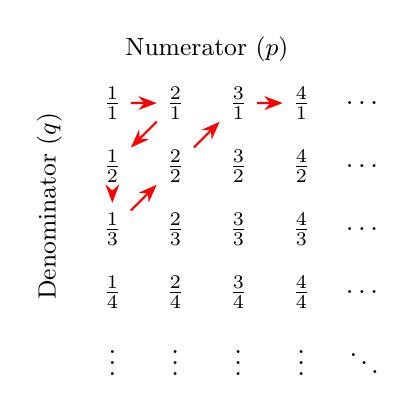
\begin{tikzpicture}[scale=0.8] % Scaled down to fit minipage
            % Draw Grid
            \foreach \x in {1,2,3,4}
                \foreach \y in {1,2,3,4}
                    \node (n\x\y) at (\x,-\y) {$\frac{\x}{\y}$};
        
            % Draw Arrows for Zig-Zag path
            \draw[red, thick, ->, >={Stealth}] (n11) -- (n21);
            \draw[red, thick, ->, >={Stealth}] (n21) -- (n12);
            \draw[red, thick, ->, >={Stealth}] (n12) -- (n13);
            \draw[red, thick, ->, >={Stealth}] (n13) -- (n22);
            \draw[red, thick, ->, >={Stealth}] (n22) -- (n31);
            \draw[red, thick, ->, >={Stealth}] (n31) -- (n41);
            
            % Label Axes
            \node[above, font=\small] at (2.5,-0.5) {Numerator ($p$)};
            \node[left, rotate=90, font=\small] at (0,-1) {Denominator ($q$)};
            \node at (5,-1) {$\dots$};
            \node at (5,-2) {$\dots$};
            \node at (5,-3) {$\dots$};
            \node at (5,-4) {$\dots$};
            \node at (5,-5) {$\ddots$};
            \node at (1,-5) {$\vdots$};
            \node at (2,-5) {$\vdots$};
            \node at (3,-5) {$\vdots$};
            \node at (4,-5) {$\vdots$};


        \end{tikzpicture}
    \end{minipage}
    \hfill
    % --- Right Minipage: Language ---
    \begin{minipage}[t]{0.48\textwidth}
        \centering
        \textbf{Countable Language ($\Sigma^2$)}
        \vspace{0.5cm}

        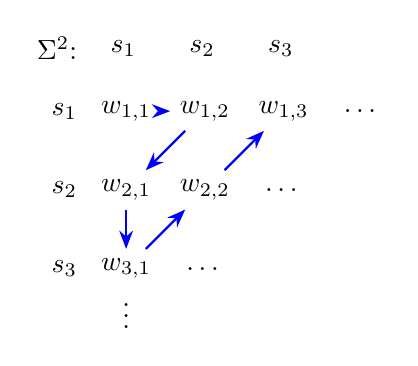
\begin{tikzpicture}[scale=1.0] % Scaled to fit minipage
            % Labels for the rows (Lengths)
            \node[anchor=east] at (0.5,-0.2) {$\Sigma^2$:};
            \node[anchor=east] at (0.5,-1) {$s_1$};
            \node[anchor=east] at (0.5,-2) {$s_2$};
            \node[anchor=east] at (0.5,-3) {$s_3$};
            \node[anchor=east] at (1.25,-0.2) {$s_1$};
            \node[anchor=east] at (2.25,-0.2) {$s_2$};
            \node[anchor=east] at (3.25,-0.2) {$s_3$};
            % Grid of strings
            \node (w11) at (1,-1) {$w_{1,1}$};
            \node (w12) at (2,-1) {$w_{1,2}$};
            \node (w21) at (1,-2) {$w_{2,1}$};
            \node (w22) at (2,-2) {$w_{2,2}$};
            \node (w31) at (1,-3) {$w_{3,1}$};
            \node (w13) at (3,-1) {$w_{1,3}$};
        
            % Path
            \draw[blue, thick, ->, >={Stealth}] (w11) -- (w12);
            \draw[blue, thick, ->, >={Stealth}] (w12) -- (w21);
            \draw[blue, thick, ->, >={Stealth}] (w21) -- (w31);
            \draw[blue, thick, ->, >={Stealth}] (w31) -- (w22);
            \draw[blue, thick, ->, >={Stealth}] (w22) -- (w13);
        
            % Dots
            \node at (4,-1) {$\dots$};
            \node at (3,-2) {$\dots$};
            \node at (2,-3) {$\dots$};
            \node at (1,-3.5) {$\vdots$};
        \end{tikzpicture}
    \end{minipage}
    \hfill
    % --- Right Minipage: Language ---
    \begin{minipage}[t]{0.48\textwidth}
        \centering
        \textbf{Countable Language ($\Sigma^{n+1}$)}
        \vspace{0.5cm}

        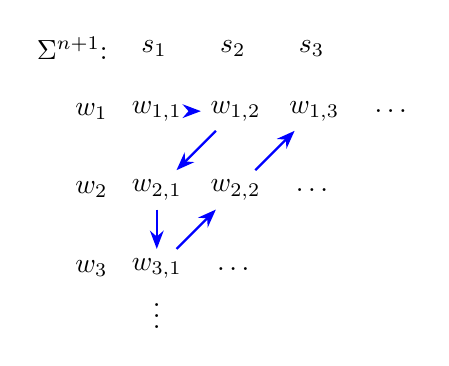
\begin{tikzpicture}[scale=1.0] % Scaled to fit minipage
            % Labels for the rows (Lengths)
            \node[anchor=east] at (0.5,-0.2) {$\Sigma^{n+1}$:};
            \node[anchor=east] at (0.5,-1) {$w_1$};
            \node[anchor=east] at (0.5,-2) {$w_2$};
            \node[anchor=east] at (0.5,-3) {$w_3$};
            \node[anchor=east] at (1.25,-0.2) {$s_1$};
            \node[anchor=east] at (2.25,-0.2) {$s_2$};
            \node[anchor=east] at (3.25,-0.2) {$s_3$};
            % Grid of strings
            \node (w11) at (1,-1) {$w_{1,1}$};
            \node (w12) at (2,-1) {$w_{1,2}$};
            \node (w21) at (1,-2) {$w_{2,1}$};
            \node (w22) at (2,-2) {$w_{2,2}$};
            \node (w31) at (1,-3) {$w_{3,1}$};
            \node (w13) at (3,-1) {$w_{1,3}$};
        
            % Path
            \draw[blue, thick, ->, >={Stealth}] (w11) -- (w12);
            \draw[blue, thick, ->, >={Stealth}] (w12) -- (w21);
            \draw[blue, thick, ->, >={Stealth}] (w21) -- (w31);
            \draw[blue, thick, ->, >={Stealth}] (w31) -- (w22);
            \draw[blue, thick, ->, >={Stealth}] (w22) -- (w13);
        
            % Dots
            \node at (4,-1) {$\dots$};
            \node at (2,-3) {$\dots$};
            \node at (3,-2) {$\dots$};
            \node at (1,-3.5) {$\vdots$};
        \end{tikzpicture}
    \end{minipage}
    % --- Right Minipage: Language ---
    \begin{minipage}[t]{0.48\textwidth}
        \centering
        \textbf{Countable Language ($\Sigma^{*}$)}
        \vspace{0.5cm}

        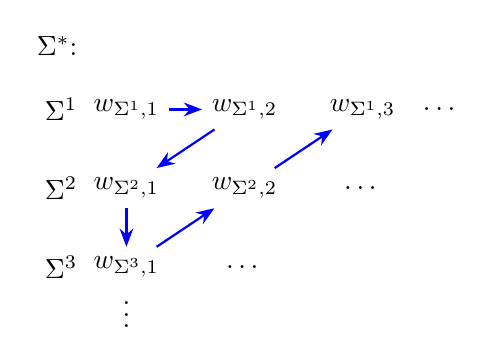
\begin{tikzpicture}[scale=1.0] % Scaled to fit minipage
            % Labels for the rows (Lengths)
            \node[anchor=east] at (0.5,-0.2) {$\Sigma^{*}$:};
            \node[anchor=east] at (0.5,-1) {$\Sigma^1$};
            \node[anchor=east] at (0.5,-2) {$\Sigma^2$};
            \node[anchor=east] at (0.5,-3) {$\Sigma^3$};
            % Grid of strings
            \node (w11) at (1,-1) {$w_{\Sigma^{1},1}$};
            \node (w12) at (2.5,-1) {$w_{\Sigma^1,2}$};
            \node (w21) at (1,-2) {$w_{\Sigma^2,1}$};
            \node (w22) at (2.5,-2) {$w_{\Sigma^2,2}$};
            \node (w31) at (1,-3) {$w_{\Sigma^3,1}$};
            \node (w13) at (4,-1) {$w_{\Sigma^1,3}$};
        
            % Path
            \draw[blue, thick, ->, >={Stealth}] (w11) -- (w12);
            \draw[blue, thick, ->, >={Stealth}] (w12) -- (w21);
            \draw[blue, thick, ->, >={Stealth}] (w21) -- (w31);
            \draw[blue, thick, ->, >={Stealth}] (w31) -- (w22);
            \draw[blue, thick, ->, >={Stealth}] (w22) -- (w13);
        
            % Dots
            \node at (5,-1) {$\dots$};
            \node at (4,-2) {$\dots$};
            \node at (2.5,-3) {$\dots$};
            \node at (1,-3.5) {$\vdots$};
        \end{tikzpicture}
    \end{minipage}
    \caption{Comparison of diagonal enumeration for numbers vs. strings.}
\end{figure}
To formalize, we use induction to prove that $\forall i \geq 0, \Sigma^i $ is countable\\
Base case: $\Sigma^1 = \Sigma$, countable as defined. \\
Inductive hypothesis: $\Sigma^n$ is countable: we enumerate all strings in $\Sigma^n$, and use the same diagonal proof to show the concatenation of 
one symbol from the countable alphabet to every string $\Sigma^{n+1}$ is also countable. Thus we can give an enumeration of all $\Sigma^i$ and use the diaganol 
argument again to show the existence of an enumeration of $\Sigma^*$. \\
Alternatively, Given 
\[\Sigma^* = \bigcup_{i\geq0} \Sigma^i\]
From the Axiom of Choice, which implies the union of countably many countable set is countable, $\Sigma^*$ is countable. 
Since $\forall L$ over $\Sigma, L \subseteq \Sigma^*, \Sigma^*$ is countable, all languages over countable $\Sigma$ is countable.
\end{proof}
\begin{definition}[Finitely Satisfiable]
    A set of formulas $\Gamma$ is said to be \textbf{finitely satisfiable} if and only if for all finite subsets $\Gamma_0 \subseteq \Gamma$, $\Gamma_0$ is satisfiable.
\end{definition}

\begin{theorem}[Compactness Theorem]
    \[ \Gamma \text{ is satisfiable} \iff \Gamma \text{ is finitely satisfiable} \]
\end{theorem}

\begin{proof}
    Consider a special case where $\Gamma$ is ``$T$-good'', defined as:
    \[ \forall p \in P, (p \in \Gamma \lor \neg p \in \Gamma) \]
    Claim: If $\Gamma$ is $T$-good, then $\Gamma \text{ is finitely satisfiable} \implies \Gamma \text{ is satisfiable}$.\\
    Suppose $\Gamma$ is $T$-good and finitely satisfiable. We define a candidate valuation $v_L$ such that for all $p \in P$:
    \[
    v_L(p) = 
    \begin{cases} 
    T & \text{if } p \in \Gamma \\ 
    F & \text{if } \neg p \in \Gamma 
    \end{cases}
    \]
    First, we prove that for every $p \in P$, \textbf{exactly one} of $\{p, \neg p\}$ is in $\Gamma$. 
    By the $T$-good property, at least one is in $\Gamma$. Suppose both $\{p, \neg p\} \subseteq \Gamma$. Consider the finite subset:
    \[ \Gamma' = \{p, \neg p\} \]
    Since $\Gamma'$ is a finite subset of a finitely satisfiable set, it must be satisfiable. However, $\neg \exists v$ such that $v \models \{p, \neg p\}$, which is a contradiction. Thus, $v_L$ is well-defined.\\\\
    Now we show $v_L \models \Gamma$. Suppose $\exists \phi \in \Gamma$ such that $v_L \not\models \phi$. Define the following finite sets based on the atoms occurring in $\phi$:
    \begin{align*}
        \Gamma_\phi^+ &= \{p \mid p \in \text{OCCUR}(\phi) \land v_L(p) = T\} \\
        \Gamma_\phi^- &= \{\neg p \mid p \in \text{OCCUR}(\phi) \land v_L(p) = F\} \\
        \Gamma_\phi &= \{\phi\} \cup \Gamma_\phi^+ \cup \Gamma_\phi^-
    \end{align*}
    Since $\Gamma_\phi$ is a finite subset of $\Gamma$, it must be satisfiable by some valuation $v$. For this $v$:
    \begin{itemize}
        \item $\forall p$ such that $p \in \Gamma_\phi^+$, $v(p) = T$.
        \item $\forall \neg p$ such that $\neg p \in \Gamma_\phi^-$, $v(\neg p) = T \implies v(p) = F$.
    \end{itemize}
    By construction, $v$ and $v_L$ agree on all atoms in $\text{OCCUR}(\phi)$. By the \textbf{Relevance Lemma}, $v(\phi) = v_L(\phi)$. 
    Since $v \models \Gamma_\phi$, we have $v \models \phi$. This implies $v_L \models \phi$, contradicting our assumption $v_L \not\models \phi$.
    Therefore, $\forall \phi \in \Gamma, v_L \models \phi$, which implies $v_L \models \Gamma$, $\Gamma$ is satisfiable.\\\\
    Now we will generalize this to all $\Gamma$ which may not be `T-good', by showing that we can construct a `T-good' finitely satisfiable set
    $\Delta$, from any finitely satisfiable $\Gamma$, and therefore show that $\Gamma SAT \iff \Delta SAT$. \\
    We will only prove the case for countable $P$ now. Let an enumeration of $p \in P$ be $\{p_1, p_2, \dots\}$\\
    Define finite subset $\Gamma_i$ of $\Gamma$ as such: 
    \begin{align*}
        &\Gamma_0 = \Gamma\\
        &\Gamma_{i+1} = \begin{cases}
            \Gamma_i \cup \{p_i\} \text{ if } \Gamma_i \cup \{p_i\} \text{ is finitely satisfiable}\\
            \Gamma_i \cup \{\neg(p_i)\} \text{ Otherwise }
        \end{cases}
    \end{align*}
    Here we need to prove that $\forall i,$ between $ \Gamma_i \cup \{p_i\}$ and $\Gamma_i \cup \{(\neg p_i)\}$ at least one case is also finitely satisfiable.
    \begin{theorem}\label{lem:fsat_union}
    Let $\Gamma$ be finitely satisfiable set, and $\phi$ be a formula, then $\Gamma \cup \{\phi\}$ is finitely satisfiable or $\Gamma \cup \{(\neg \phi)\}$ 
    is finitely satisfiable.
    \end{theorem}
    \begin{proof}
        We prove the contrapositive of this statement: if $\Gamma \cup \{\phi\}$ and $\Gamma \cup \{(\neg \phi)\}$ are both not finitely satisfiable, $\Gamma$
        is not fintely satisfiable. Given both are not finitely satisfiable, there exist finite subsets $\Gamma_1, \Gamma_2 \subseteq \Gamma$ such that 
        $\Gamma_1 \cup \{\phi\}$ and $\Gamma_2 \cup \{(\neg \phi)\}$ are not satisfiable. Therefore for all valuations, it must not model either $\Gamma_1$ or $\{\phi\}$, and not model 
        either $\Gamma_2$ or $\{(\neg \phi)\}$. Denote the set of valuations that models formula $\psi$ as $models(\psi)$, the set of valuations that models set of formula $\Sigma$ as $models(\Sigma)$
        \begin{align*}
            models(\Gamma_1) &\cap models(\phi) = \emptyset\\
            &\rightarrow \forall v \in models(\Gamma_1), v\not \models \phi \rightarrow v \models (\neg \phi)\\
            &\rightarrow models(\Gamma_1) \subseteq models((\neg \phi))\\
            models(\Gamma_2) &\cap models((\neg \phi)) = \emptyset\\
            &\rightarrow \forall v \in models(\Gamma_2), v\not \models (\neg \phi) \rightarrow v \models (\phi)\\
            &\rightarrow models(\Gamma_2) \subseteq models(\phi)\\
        \end{align*}
        Now consider the set of valuations that models $\Gamma_1 \cup \Gamma_2$
        \begin{align*}
            &models(\Gamma_1 \cup \Gamma_2) = models(\Gamma_1) \cap models(\Gamma_2)\\
            &(models(\Gamma_1) \cap models(\Gamma_2)) \subseteq (models(\phi) \cap models((\neg \phi))) = \emptyset\\
        \end{align*}
        Since $\Gamma_1 \cup \Gamma_2$ is a finite subset of $\Gamma$ that is not satisfiable, $\Gamma$ is not finitely satisfiable. 
    \end{proof}
    Now prove that 
    \begin{lemma}\label{lem:fsat_each}
    $\forall i, \Gamma_i$ is finitely satisfiable.     
    \end{lemma}
    \begin{proof}
        Base case: 
        \[\Gamma_0 = \Gamma \text{ is finitely satisfiable by definition}\]
        Inducetive hypothesis: Suppose
        \[\Gamma_n \text{ is finitely satisfiable}\]
        By Lemma~\ref{lem:fsat_union}, $\Gamma_n \cup \{p_n\}$ and $\Gamma_n \cup \{(\neg p_n)\}$ there must be at least one that is finitely satisfiable.
        $\rightarrow$ $\Gamma_{n+1}$ is therefore finitely satisfiable.
    \end{proof}
    Next we will show that 
    \begin{lemma}\label{lem:fsat_all}
    $\Gamma_U = \bigcup_{i\geq0} \Gamma_i$ is finitely satisfiable.    
    \end{lemma}
    \begin{proof}
        Consider finite set $\Gamma' \subseteq \Gamma_U$, since $\Gamma'$ is finite, and $\forall k\geq 0, \Gamma_k \subseteq \Gamma_{k+1}$ by definition,
        $\exists j \geq 0, \Gamma' \subseteq \Gamma_j = \bigcup_{i\geq 0}^j \Gamma_i$. By Lemma~\ref{lem:fsat_each}, $\Gamma_j$ is satisfiable $\rightarrow \Gamma'$ is finitely satisfiable.
    \end{proof}
    \begin{lemma}\label{lem:const_sat}
        $\Gamma_U$ is satisfiable.
    \end{lemma}
    \begin{proof}
        From the construction, $\forall i \geq 0$ at least one of $p_i$ and $(\neg p_i)$ is in $\bigcup_{i\geq 0} \Gamma_i$. Since $\bigcup_{i\geq 0} \Gamma_i$ is finitely satisfiable, 
        $\forall i \geq 0, p_i$ and $(\neg p_i)$ cannot both be in $\bigcup_{i\geq 0} \Gamma_i$. Otherwise $\{p_i\} \cup \{(\neg p_1)\} \subseteq \bigcup_{i\geq 0} \Gamma_i$ is not satisfiable, contradiction.
    \end{proof}
    Now we have proven that the construction proposed from a finitely satisfiable formula set $\Gamma$ to $\bigcup_{i\geq 0} \Gamma_i$ is also finitely satisfiable. Now to complete the proof of
    the compactness theorem, we need to prove that $\exists v, v\models \Gamma$.
    \begin{proof}
        From Lemma~\ref{lem:const_sat}, 
        $\forall i\geq 0, (p_i \in \Gamma_U) 
        \oplus ((\neg p_i) \in \Gamma_U)$, $\exists v, v \models \Gamma_U$
        \[v(p):P \mapsto \{T, F\} = \begin{cases}
            T, \text{ if } p \in \Gamma_U\\
            F, \text{ if } (\neg p) \in \Gamma_U
        \end{cases}\]
        Define the literal set $Literals = \{p_i, (\neg p_i) \mid i \geq 0\}$, 
        and function 
        \[\tau(p): P \mapsto Literals = \begin{cases}
            p, \text{ if } p \in \Gamma_U\\
            (\neg p), \text{ if } (\neg p) \in \Gamma_U
        \end{cases}\]
        \begin{lemma}
            \[v\models \Gamma_U \rightarrow v \models \tau(\Gamma)\]
        \end{lemma}
        Let $\phi \in \Gamma$, Define literal set $X = \{\tau(p) \mid p \in OCCUR(\phi)\}$
        where $X$ is a set containing single proposition literals. 
        By definition we have 
        \[X \subseteq \Gamma_U \rightarrow v \models X \rightarrow \forall \psi \in X, v(\psi) = T\]
        and $OCCUR(X) = OCCUR(\phi)$
        Since both $X$ is finite, $X \cup \{\phi\}$ is a finite subset to $\Gamma_U$, thus satisfiable. 
        $\rightarrow \exists v', v' \models X\cup \{\phi\} \rightarrow v' \models X, v' \models \phi \rightarrow
        \forall \psi \in X, v'(\psi) = T$. 
        \[\forall p \in OCCUR(\phi), v(p) = v'(p), v' \models \phi \rightarrow v\models \phi\]
        Therefore, the valuation that models enlarged construction $\Gamma_U$ also models $\Gamma$, thus $\Gamma$ 
        is satisfiable.
    \end{proof}
\end{proof}

\subsection{Application of the Compactness theorem for proposition logics}
We have already shown that we can use propositional logic to model computational problems, the compactness theorem allows us to extend 
problem modelling to instances of infinite size. Recall the k-colorable problem, where we used propositional logic to model any finite size
instance. 
\begin{theorem}
    A graph is k-colorable iff every finite subgraph is k-colorable.
\end{theorem}
\begin{definition}[Infinite graph]
    $G = (V, E)$ is an infinite graph if $V$ is infinite.
\end{definition}
\begin{definition}[Subgraph]
    $G' = (V', E')$ is a subgraph to $G$ if $V' \subseteq V, E' \subseteq E$
\end{definition}
\begin{definition}[Induced subgraph]
    $G' = (V', E')$ is an induced subgraph to $G$ if $G'$ is a subgraph to $G$, and $\{u, v\} \in E' \iff \{u, v\} \in E \land u, v \in V'$
\end{definition}
\begin{proof}
Since we have formulated any finite instance of k-colorable graph as propositional logic formula, we can define infinite set 
\[\Gamma_G = \{\phi_{G'}^{k-colorable}\mid G' \text{ is finite subgraph of } G\}\]
We will first prove that 
    \begin{lemma}
        $G$ is finitely k-colorable $\rightarrow$ $\Gamma_G$ is finitely satisfiable.
    \end{lemma}
    \begin{proof}
        We will reuse the proposition definition from last chapter, where $|V|$ and thus $P$ is countable
    \[P = \{p_{v, i} \mid v \in V, i \in [1, k]\}\]
        For each instance on $G = (V, E)$ and $k$ colors, we formulate as such to enforce constraints on edges (No same color on adjacent vertices),
        and vertices (exactly 1 coloring on each vertex).
        \[\phi = \phi^{nbr} \land \phi^{exactly-1-color}\]
        Consider the infinite graph $G = (V, E)$
        \begin{align*}
            \Gamma_G &= \Gamma^{nbr}_G \cup \Gamma^{exactly-1-color}_G\\
            \Gamma^{exactly-1-color}_G &= \{\phi^{exactly-1-color}_v \mid v \in V\}\\
            \phi^{exactly-1-color}_{v} &= (\bigvee_{i \in [1, k]}p_{v, i}) \land (\bigwedge_{i \neq j \in [1, k]} (p_{v, i} \rightarrow p_{v, j}))\\
            \Gamma^{nbr}_G &= \{\phi^{nbr}_{\{u, v\}} \mid \{u, v\} \in E\}\\
            \phi^{nbr}_{\{u, v\}} &= \bigwedge_{i \in [1, k]}(p_{u, i} \rightarrow p_{v, i})
        \end{align*}

    Suppose the contrary, where $G = (V, E)$ is finitel k-colorable, $\Gamma_G$ is not finitely satisfiable, 
    $\exists$ finite subset $ \Gamma_0 \subseteq \Gamma_G, \Gamma_0$ is not satisfiable. 
    Let $G_0 = (V_0, E_0)$ be a finite subgraph of $G$, such that 
    \[V_0 = \{v \mid v \in V, \phi^{exactly-1-color}_v \in \Gamma_0\} \cup \{u \mid u \in V, \exists u', \phi^{nbr}_{\{u, u'\}} \in \Gamma_0\}\]
    \[E_0 = \{\{u, v\} \mid \{u, v\} \in E, u, v \in V_0\}\]
    Here we are formulating an instance of finite k-colorable induced subgraph of $G$ from finite subset $\Gamma_0$. Now we need to show that $G_0$ is not k-colorable
    to reach the contradiction, with another contradiction. \\
    Suppose $G_0$ is k-colorable, let $C_0$ be a k-coloring of $G_0$, define valuation
    \[v_0(p_{u, i}) =\begin{cases}
        T, \text{ if } C_0(u) = i\\
        F, \text{ if } C_0(u) \neq i
    \end{cases} \]
    Let \[\Gamma_0' = \{\phi^{exactly-1-color}_v \mid v \in V_0\} \cup \{\phi^{nbr}_{\{u, v\}} \mid \{u, v\} \in E_0\}\]
    Consider 

    \[\Gamma_0 \subseteq \Gamma_0'\] %how?%
    Since $\Gamma_0'$ is the same construction from k-colorability to formuala, $G_0$ is k-colorable, we have 
    \[v_0 \models \Gamma_0'\]
    By relevance lemma
    \[v_0 \models \Gamma_0\]
    Contradicting to our initial assumption that $\Gamma_0$ is NOT satisfiable. 
    \end{proof}
By Compactness theorem, $\Gamma_G$ is finitely satisfiable $\rightarrow \Gamma_G$ is 
satisfiable.
    \begin{lemma}
        $\Gamma_G$ is satisfiable $\rightarrow G$ is k-colorable 
    \end{lemma}
    \begin{proof}
        $\Gamma_G$ is satisfiable $\rightarrow \exists v, v\models \Gamma_G$. We can construct a coloring $C$ from $v$ 
        similarly to how we constructed $v_0$ from $C_0$ from previous proof:
        \[C(v) = i, \text{ if } v(p_{v, i}) = T\]
        By construction the coloring is valid, detailed technicality is ommitted.
    \end{proof}
\end{proof}

\subsection{Proof of König's Lemma via Compactness}König's Lemma states that every infinite, finitely branching tree contains an infinite path. We can prove this elegantly using the Compactness Theorem for Propositional Logic, which states that a set of formulas $\Gamma$ is satisfiable if and only if every finite subset of $\Gamma$ is satisfiable.\begin{theorem}[König's Lemma]Let $T$ be a tree with an infinite number of vertices such that every vertex has a finite degree (finitely branching). Then $T$ contains at least one infinite path starting from the root.\end{theorem}\begin{proof}To prove this using propositional logic, we define a set of propositional variables and constraints that force the existence of an infinite path.\textbf{1. Define Propositional Variables:}For every vertex $v \in T$, let $P_v$ be a propositional variable. The intended meaning is:$$ P_v \text{ is true} \iff v \text{ is part of the infinite path.} $$\textbf{2. Construct the Set of Formulas $\Gamma$:}We include the following requirements in our set $\Gamma$:\begin{itemize}\item \textbf{Existence at each level:} For each natural number $n$, at least one vertex at depth $n$ must be on the path.$$ \bigvee_{v \in Level(n)} P_v $$(Note: This is a finite disjunction because the tree is finitely branching.)\item \textbf{Uniqueness per level:} No two distinct vertices $u, v$ at the same level can both be on the path.$$ \neg (P_u \land P_v) \quad \text{for } u, v \in Level(n), u \neq v $$\item \textbf{Structure (Parental Link):} If a vertex $v$ (at depth $> 0$) is on the path, its unique parent $u$ must also be on the path.$$ P_v \rightarrow P_u $$\end{itemize}\textbf{3. Apply Compactness:}Consider any finite subset $\Gamma_0 \subseteq \Gamma$. Let $N$ be the maximum depth of any vertex mentioned in $\Gamma_0$. Since the tree is infinite and finitely branching, there must be at least one vertex $v_{max}$ at depth $N$. We can satisfy $\Gamma_0$ by picking $v_{max}$ and its ancestors back to the root, setting those variables to \textit{true} and all others to \textit{false}.Since every finite subset $\Gamma_0$ is satisfiable, the Compactness Theorem implies that the entire set $\Gamma$ is satisfiable.\textbf{4. Conclusion:}Let $\mathcal{I}$ be a satisfying assignment for $\Gamma$. The set of vertices $V_{path} = \{v \in T \mid \mathcal{I}(P_v) = \text{true}\}$ defines a sequence of vertices starting from the root where each level has exactly one vertex, and each vertex is connected to its parent. This sequence forms an infinite path.\end{proof}
\section{Proof System}
\subsection{Hilbert Style Proof System }
Four axiom schema of the hilberts style proof system. Axiom schema means that the $\phi, \psi, \rho$ in these schema are placehoders that 
can be replaced by any valid formula
\begin{enumerate}

    \item Axiom 1: Simplification
    \begin{prooftree}
        \AxiomC{}
        \UnaryInfC{$p \to (q \to p)$}
    \end{prooftree}
    
    \item Axiom 2: Distribution
    \begin{prooftree}
        \AxiomC{}
        \UnaryInfC{$(p \to (q \to r)) \to ((p \to q) \to (p \to r))$}
    \end{prooftree}
    
    \item Axiom 3: Double Negation Elimination (DNE)
    \begin{prooftree}
        \AxiomC{}
        \UnaryInfC{$((p \to \bot) \to \bot) \to p$}
    \end{prooftree}
    
    \item Rule of Inference: Modus Ponens
    \begin{prooftree}
        \AxiomC{$p \to q$}
        \AxiomC{$p$}
        \BinaryInfC{$q$}
    \end{prooftree}
\end{enumerate}
The horizontal lines are judgement lines, which means that whats below can be inferred from whats above. The first 3 rules has no assumptions or 
premises, meaning they are ways we can introduce arbituary claims or assumption into our proofs. 
\begin{definition}[Proof]
    A proof of the consequence of $\phi$ from $\Gamma$ is a finite sequence of formula $c_1, c_2, \dots, c_k$ where 
    $\forall i \leq k, c_i \in \Gamma$ or, $c_i$ is obtained using one of the 4 axioms:
    \begin{itemize}
        \item $\exists j, l < i, c_j \equiv c_l \rightarrow c_i$
        \item $\exists \phi, \psi, c_i \equiv \phi \rightarrow (\psi \rightarrow \phi)$
        \item $\exists \phi, \psi, \rho, c_i \equiv [\phi \rightarrow (\psi \rightarrow \rho)] \rightarrow [(\phi \rightarrow \psi) \rightarrow (\phi \rightarrow \rho)]$
        \item $\exists \phi, c_i \equiv ((\phi \rightarrow \bot) \rightarrow \bot)\rightarrow \phi$
    \end{itemize}
\end{definition}
\begin{definition}[Derivable]
    $\phi$ is derivable from $\Gamma$ if there is a proof in HSPS of "$\phi$ is a consequence of $\Gamma$"
    \[\Gamma \vdash \phi\]
\end{definition}
\begin{example}
\[\Gamma = \{p, p\rightarrow q\}, \quad \phi = q\]
\begin{proof}
    We can construct proof sequence:
    \begin{align*}
        c_1 &= p                && (p \in \Gamma) \\
        c_2 &= p \to q          && (p \to q \in \Gamma) \\
        c_3 &= q                && (\text{Modus Ponens on } c_1, c_2)
    \end{align*}
\end{proof}
\end{example}
Sometimes HSPS requires us to creatively introduce new hypothesis to assist in the proof.
\begin{example}
    \[\Gamma = \{\bot\}, \phi = p\]
    Intuitively this does not sound provable, just from $\bot$, but axioms that require no premises allows us to introduce helper hypothesis. In this case
    $(p \rightarrow \bot)$
    \begin{proof}
        \begin{align*}
            c_1 &= \bot                && (\bot \in \Gamma) \\
            c_2 &= \bot \rightarrow [(p\rightarrow \bot) \rightarrow \bot]          && (\text{Axiom 1: Simplification}) \\
            c_3 &= (p\rightarrow \bot) \rightarrow \bot                && (\text{Modus Ponens on } \bot, (p \rightarrow \bot))\\
            c_4 &= [(p\rightarrow \bot) \rightarrow \bot] \rightarrow p && (\text{Axiom 3: Double negation})\\
            c_5 &= p && (\text{Modus Ponens on } c_3 \equiv [(p \rightarrow \bot) \rightarrow \bot], c_4 \equiv ([(p\rightarrow \bot) \rightarrow \bot] \rightarrow p))
        \end{align*} 
    \end{proof}
\end{example}
As seen from  this example, HSPS can get convoluted and unintuitive for relatively straightforward consequences. 
\subsubsection*{1. Self-Implication: $\vdash p \to p$}

\paragraph{Idea.}
We must simulate identity using only distribution.

\begin{enumerate}
    \item $p \to ((p \to p) \to p)$ \hfill (Axiom 1)
    \item $p \to (p \to p)$ \hfill (Axiom 1)
    \item $(p \to ((p \to p) \to p)) \to ((p \to (p \to p)) \to (p \to p))$ \hfill (Axiom 2)
    \item $(p \to (p \to p)) \to (p \to p)$ \hfill (MP 1,3)
    \item $p \to p$ \hfill (MP 2,4)
\end{enumerate}

Even the trivial tautology requires a nontrivial derivation.

\bigskip
\subsubsection*{2. Contraposition: $\vdash (p \to q) \to ((q \to \bot) \to (p \to \bot))$}

\paragraph{Idea.}
Assume $p \to q$ and $q \to \bot$; derive $p \to \bot$ via Axiom 2.

\begin{enumerate}
    \item $(p \to (q \to \bot)) \to ((p \to q) \to (p \to \bot))$ \hfill (Axiom 2)
    \item $(q \to \bot) \to (p \to (q \to \bot))$ \hfill (Axiom 1)
    \item $(p \to q) \to ((q \to \bot) \to (p \to \bot))$
\end{enumerate}

The last line follows by two applications of Modus Ponens
using (1) and (2).

This shows implication reversal must be encoded indirectly.

\bigskip
\subsubsection*{3. Peirce’s Law: $\vdash ((p \to q) \to p) \to p$}

This formula characterizes classical logic.

\paragraph{Sketch.}

\begin{enumerate}
    \item $((p \to q) \to p) \to (((p \to q) \to p) \to ((p \to q) \to p))$ \hfill (Ax1)
    \item Use Axiom 2 repeatedly to simulate assumption chaining.
    \item Derive $(((p \to q) \to p) \to \bot) \to \bot$.
    \item Apply Axiom 3 (DNE) to conclude $((p \to q) \to p) \to p$.
\end{enumerate}

The essential trick:
Peirce’s law is obtained by embedding the formula into
a double-negation context and applying Axiom 3.

This is far from syntactically obvious.

\bigskip
\subsubsection*{4. Explosion: $\vdash \bot \to p$}

In this system $\bot$ is primitive via $p \to \bot$.

\paragraph{Idea.}
Show that from $\bot$ we can derive anything.

\begin{enumerate}
    \item $p \to (\bot \to p)$ \hfill (Ax1)
    \item $\bot \to (p \to \bot)$ \hfill (Ax1)
    \item $(\bot \to (p \to \bot)) \to ((\bot \to p) \to (\bot \to \bot))$ \hfill (Ax2)
    \item Derive $\bot \to \bot$ using the $p \to p$ pattern.
    \item Conclude $\bot \to p$.
\end{enumerate}

Notice how even explosion must be simulated through distribution.

\bigskip
\subsubsection*{5. Double Negation Introduction: $\vdash p \to ((p \to \bot) \to \bot)$}

Although Axiom 3 gives elimination,
introduction must be derived.

\begin{enumerate}
    \item $(p \to \bot) \to (p \to (p \to \bot))$ \hfill (Ax1)
    \item Use Axiom 2 to rearrange implication nesting.
    \item Conclude $p \to ((p \to \bot) \to \bot)$.
\end{enumerate}

This illustrates asymmetry between DNE and its converse.

\subsection{Metatheorems}
\subsubsection{Monotonicity theorem}
\begin{theorem}
\[\Gamma \vdash A, \Gamma \subseteq \Delta \implies \Delta \vdash A\]    
\end{theorem}
\begin{proof}
    Let the proof of $A$ from $\Gamma$ be the sequence $\langle \phi_1, \phi_2, \dots, \phi_n\rangle, \phi_n = A$
    \subsubsection*{Base case: $n = 1$}
    \begin{itemize}
        \item Case 1: $\phi_1 \in \Gamma \implies \phi_1 \in \Delta \implies \Delta \vdash \phi_1$
        \item Case 2: $\phi_1$ is from one of the axiom schema, $\Delta \vdash \phi_1$
    \end{itemize}
    \subsubsection*{Inductive step: $\forall i < n, \Gamma \vdash \phi_i, \Delta \vdash \phi_i$}
    \begin{itemize}
        \item Case 1, 2: $\phi_{i+1} \in \Gamma$ or $\phi_{i+1}$ is from one of the axiom schema, trivial
        \item Case 3: $\phi_{i+1}$ is from Modus Ponens, $\exists \phi_j$ such that 
        \begin{prooftree}
            \AxiomC{$\phi_j \to \phi_{i+1}$}
            \AxiomC{$\phi_j$}
            \BinaryInfC{$\phi_{i+1}$}
        \end{prooftree}
        $\Gamma \vdash \phi_j, \Gamma \vdash \phi_j \rightarrow \phi_{i+1}$ by inductive hypothesis, $\Delta \vdash \phi_j, \Delta \vdash \phi_j \rightarrow \phi_{i+1}$, by MP, $\Delta \vdash \phi_{i+1}$
    \end{itemize}
\end{proof}
\subsubsection{Deduction}
\begin{theorem}
\[\Gamma \cup \{A\} \vdash B \iff \Gamma \vdash A \rightarrow B\]
\end{theorem}
\begin{proof}
    \subsubsection*{$(\implies)$}
    We will use structural induction over the length of derivation from $\Gamma \cup \{A\}$ to $B$, 
    $\Gamma \cup \{A\} \vdash B \implies \exists \langle \phi_1, \phi_2, \dots, \phi_n\rangle, \phi_n = B$.
    \subsubsection*{Base case: $n = 1, \phi_n = B$}
    \begin{itemize}
        \item Case 1: $B$ is an axiom $\Gamma \vdash B$. By simplification axiom, $\Gamma \vdash B \rightarrow (A \rightarrow B)$, by MP, $\Gamma \vdash A\rightarrow B$.
        \item Case 2: $B = A$, we will use the simplification and distribution axioms:
        \begin{itemize}
            \item $p \equiv A$
            \item $q \equiv (A\rightarrow A)$
            \item $r \equiv A$
        \end{itemize}
        \begin{itemize} 
            \item $(A\rightarrow ((A \rightarrow A)\rightarrow A)) \rightarrow ((A\rightarrow (A \rightarrow A))\rightarrow (A \rightarrow A))$ (Distribution)
            \item $A\rightarrow((A\rightarrow A)\rightarrow A)$ (Simplification)
            \item $(A\rightarrow(A\rightarrow A)) \rightarrow(A \rightarrow A)$ (MP)
            \item $A \rightarrow(A \rightarrow A)$ (Simplification)
            \item $(A \rightarrow A)$ (MP)
        \end{itemize}
        $\Gamma \vdash A \rightarrow A \implies \Gamma \vdash A \rightarrow B$
    \end{itemize}
    \subsubsection*{Inductive step: Suppose $\forall i < n, \Gamma \cup \{A\} \vdash \phi_i \implies \Gamma \vdash A\rightarrow \phi_i$}
    \begin{itemize}
        \item Case 1, 2, 3: $\phi_{i+1}$ is in $\Gamma$ or $\phi_{i+1}$ is from one of the axioms, trivial; If $\phi_{i+1} = A$, the same as Case 2 in base case
        \item Case 4: $\phi_{i+1}$ is obtained from MP, where $\exists j \leq i$, 
        \begin{align*}
        &\Gamma\cup \{A\} \vdash \phi_j &&\implies \Gamma \vdash A \rightarrow \phi_j\\
        &\Gamma\cup \{A\} \vdash \phi_{j} \rightarrow \phi_{i+1} &&\implies \Gamma \vdash A \rightarrow (\phi_j \rightarrow \phi_{i+1})
        \end{align*}
        \begin{prooftree}
            \AxiomC{$\phi_j \to \phi_{i+1}$}
            \AxiomC{$\phi_j$}
            \BinaryInfC{$\phi_{i+1}$}
        \end{prooftree}
        \begin{align*}
            &\Gamma \vdash (A \rightarrow \phi_j) \rightarrow (A \rightarrow \phi_{i+1}) && \text{ by distribution}\\
            &\Gamma \vdash A \rightarrow \phi_{i+1} && \text{ by MP}
        \end{align*}
    \end{itemize}
\end{proof}
\begin{theorem}[Soundness of HSPS]
    HSPS is sound. 
    \[\Gamma \vdash \phi \implies \Gamma \models \phi\]
\end{theorem}
\begin{proof}
    Define property $H(i): \forall j\leq i, \Gamma \models c_j$.\\
    \subsubsection*{Base case: $i = 1$}
    Suppose $\Gamma \vdash \phi, \exists \pi = c_1, c_2, \dots, c_k, c_k = \phi$. 
    By definition, $c_1 \in \Gamma$ or 
    \begin{itemize}
        \item $\exists \phi, \psi, c_1 \equiv \phi \rightarrow (\psi \rightarrow \phi)$
        \item $\exists \phi, \psi, \rho, c_1 \equiv [\phi \rightarrow (\psi \rightarrow \rho)] \rightarrow [(\phi \rightarrow \psi) \rightarrow (\phi \rightarrow \rho)]$
        \item $\exists \phi, c_1 \equiv ((\phi \rightarrow \bot) \rightarrow \bot)\rightarrow \phi$
    \end{itemize}
    Note that Modus Ponens is not possible to yield $c_1$ as we need at least 1 previous formula.\\
    If $c_1 \in \Gamma, \Gamma \models c_1$; Else, if $c_1$ comes from any other axiom, $c_1$ is valid, i.e. $\forall v, v\models c_1$, therefore $\Gamma \models c_1$
    \subsubsection*{Inductive step:}
    Suppose $H(i), \forall j < i, \Gamma \models c_j, \forall v \models \Gamma, v \models c_j$.
    \begin{itemize}
        \item Case 1, 2: $c_{i+1} \in \Gamma$, or $c_{i+1}$ is from an axiom, $\Gamma \models c_{i+1}, H(i+1)$
        \item Case 3: $c_{i+1}$ comes from MP: $\exists j < i, \Gamma \vdash c_j, \Gamma \vdash c_j \rightarrow c_{i+1}$. By inductive hypothesis, $\forall v \models \Gamma, 
        v\models c_j, v \models c_j \rightarrow c_{i+1}$
        \begin{align*}
            &v(c_j) = T\\
            &v(c_j \rightarrow c_{i+1}) = T \equiv v(\neg c_j \lor c_{i+1}) = T\\
            &\quad \quad v(\neg c_j) = T \text{ OR } v(c_{i+1}) = T\\
            &v(c_j) = T \implies v(\neg c_j) = F \implies v(c_{i+1}) = T \\
            &\implies \forall v \models \Gamma, v\models c_{i+1} \implies \Gamma \models c_{i+1}
        \end{align*}
    \end{itemize}
\end{proof}
\begin{theorem}[Completeness of HSPS]
    HSPS is complete. 
    \[\Gamma \models \phi \implies \Gamma \vdash \phi\]
\end{theorem}

{\color{blue}
    \subsection{Weak Completeness and Completeness of HSPS}

We work with the Hilbert-Style Propositional System (HSPS):

\begin{itemize}
    \item Axiom 1: $p \to (q \to p)$
    \item Axiom 2: $(p \to (q \to r)) \to ((p \to q) \to (p \to r))$
    \item Axiom 3: $((p \to \bot) \to \bot) \to p$
    \item Rule: Modus Ponens
\end{itemize}

We write $\vdash \varphi$ for provability and $\models \varphi$ for semantic validity.

\bigskip
\subsubsection*{1. Weak Completeness}

\begin{theorem}[Weak Completeness]
If $\models \varphi$, then $\vdash \varphi$.
\end{theorem}

\paragraph{Idea.}
We prove the contrapositive: if $\nvdash \varphi$, then $\not\models \varphi$.
That is, if $\varphi$ is not provable, then there exists a valuation falsifying it.

\paragraph{Step 1: Consistency and Maximal Consistency.}

A set $\Gamma$ is \emph{consistent} if $\Gamma \nvdash \bot$.

If $\nvdash \varphi$, then $\{\neg \varphi\}$ is consistent.

Using a standard Lindenbaum construction:

\begin{itemize}
    \item Extend any consistent set $\Gamma$
    \item to a \emph{maximal consistent set} $\Delta$
    \item such that for every formula $\psi$:
    \[
    \psi \in \Delta \quad \text{or} \quad \neg \psi \in \Delta.
    \]
\end{itemize}

This construction relies only on classical logic and
the deduction theorem (derivable in HSPS).

\paragraph{Step 2: Canonical Valuation.}

Define a valuation $v_\Delta$ by:

\[
v_\Delta(p) =
\begin{cases}
\text{true} & \text{if } p \in \Delta \\
\text{false} & \text{otherwise}
\end{cases}
\]

We prove by structural induction:

\[
\psi \in \Delta
\quad \Longleftrightarrow \quad
v_\Delta \models \psi.
\]

The key steps use:

\begin{itemize}
    \item Maximality of $\Delta$
    \item Closure under Modus Ponens
    \item Axiom 3 for classical negation
\end{itemize}

\paragraph{Step 3: Falsifying $\varphi$.}

Since $\neg \varphi \in \Delta$,
we obtain:

\[
v_\Delta \models \neg \varphi,
\quad\text{hence}\quad
v_\Delta \not\models \varphi.
\]

Therefore $\varphi$ is not valid.

\paragraph{Conclusion.}

\[
\models \varphi \;\Longrightarrow\; \vdash \varphi.
\]

\hfill $\square$

\bigskip
\subsubsection*{2. Strong Completeness (Full Completeness)}

\begin{theorem}[Completeness]
If $\Gamma \models \varphi$, then $\Gamma \vdash \varphi$.
\end{theorem}

\paragraph{Reduction to Weak Completeness.}

Suppose $\Gamma \models \varphi$.

Then:
\[
\models \bigwedge \Gamma \to \varphi.
\]

If $\Gamma$ is finite, we directly apply weak completeness:

\[
\vdash (\bigwedge \Gamma) \to \varphi.
\]

Repeated applications of Modus Ponens yield:

\[
\Gamma \vdash \varphi.
\]

\paragraph{Infinite Case.}

If $\Gamma$ is infinite:

\begin{itemize}
    \item If $\Gamma \models \varphi$,
    \item then some finite subset $\Gamma_0 \subseteq \Gamma$
    satisfies $\Gamma_0 \models \varphi$
    (compactness of propositional logic).
\end{itemize}

Apply the finite case to $\Gamma_0$,
then use monotonicity of derivability:

\[
\Gamma \vdash \varphi.
\]

\bigskip
\subsubsection*{3. Conceptual Structure}

Weak completeness:
\[
\models \varphi \Rightarrow \vdash \varphi.
\]

Strong completeness:
\[
\Gamma \models \varphi \Rightarrow \Gamma \vdash \varphi.
\]

The essential engine is:

\begin{enumerate}
    \item Maximal consistent sets
    \item Canonical valuation
    \item Truth lemma
\end{enumerate}

Axiom 3 ensures classicality, making the canonical model work.

\bigskip
\subsubsection*{4. Final Picture}

Soundness:
\[
\vdash \varphi \Rightarrow \models \varphi.
\]

Completeness:
\[
\models \varphi \Rightarrow \vdash \varphi.
\]

Hence:

\[
\vdash \varphi
\quad \Longleftrightarrow \quad
\models \varphi.
\]

HSPS is therefore sound and complete for classical propositional logic.

\hfill $\blacksquare$
}




\subsection{Resolution Proof System}
\begin{definition}[Clause]
    For each proposition $p$ define literals $p$ and $\neg p$. A clause $C$ is finite set of literals over the proposition set $P$. 
    \[v \models C = \{\ell_1, \ell_2, \dots, \ell_k\} \iff \exists j, v\models \ell_j\]
    As such, a cluase $C$ is satisfiable if $\exists v, v\models C$
\end{definition}
Note that from this defintion, an empty clause (an empty set of literals) is not satisfiable, as intuitively, a valuation models a clause if 
there exists at least one literal in the clause such that $v\models \ell$.
\begin{definition}[Conjunctive normal form (CNF)]
A formula $\phi$
is said to be in Conjunctive Normal Form is 
\[\phi \equiv \bigwedge_{i=1}^k C_i\]
\end{definition}
\subsubsection*{}
\begin{definition}[Satisfiability of a set of clauses]
\[\Gamma = \{C_1, C_2, \dots\}\]
\begin{itemize}
    \item $\Gamma$ is satisfiable if $\exists v, \forall C\in \Gamma, v\models C$
    \item $\Gamma$ is unsatisifiable if $\forall v, \exists C\in \Gamma,  v\not \models C$
\end{itemize}
\end{definition}
By this definition,
\begin{itemize}
    \item $\Gamma = \emptyset$ is vacuously satisfiable
    \item $\Gamma = \{\emptyset\}$ is not satisifiale. 
    \item Any set of clauses that contains the empty set is unsatisfiable
\end{itemize}
\begin{theorem}
    Each well-formed formula can be transformed to a logically equivalent CNF
\end{theorem}
\begin{proof}
\subsubsection*{Base case: $\phi \in P$}
trivial
\subsubsection*{Inductive Case 1: $\neg$ }
Suppose there exists a CNF $\bigwedge_i \bigvee_j \ell_{i, j}$ logically equivalent to $\phi$. 
\begin{align*}
    \neg \phi &= \neg ((\ell_{1,1}\lor \ell_{1, 2}\lor \dots) \land (\ell_{2, 1}\lor \ell_{2, 2} \lor \dots ) \land \dots)\\
    &=\neg(\ell_{1,1}\lor \ell_{1, 2}\lor \dots) \lor \neg(\ell_{2, 1}\lor \ell_{2, 2} \lor \dots ) \lor \dots\\
    &=(\neg \ell_{1,1}\land \neg\ell_{1, 2}\land \dots) \lor (\neg\ell_{2, 1}\land \neg\ell_{2, 2} \land \dots ) \lor \dots\\
    &= (\neg \ell_{1,1} \lor \neg \ell_{2, 1} \lor \dots) \land ()
\end{align*}
\subsubsection*{Inductive Case 2: $\land$}
Suppose $\phi \equiv \bigwedge_{i \in I} C_i$ and $\psi \equiv \bigwedge_{j \in J} D_j$ are CNFs.
\begin{align*}
    \phi \land \psi &\equiv \left( \bigwedge_{i \in I} C_i \right) \land \left( \bigwedge_{j \in J} D_j \right) \\
    &\equiv \bigwedge_{k \in I \cup J} E_k
\end{align*}
where $E_k$ is a clause from the set of clauses of $\phi$ or $\psi$. Since the conjunction of two conjunctions is simply a larger conjunction of the original clauses, the result is by definition a CNF.

\subsubsection*{Inductive Case 3: $\lor$}
Suppose $\phi \equiv \bigwedge_{i \in I} C_i$ and $\psi \equiv \bigwedge_{j \in J} D_j$ are CNFs. By applying the Distributive Law:
\begin{align*}
    \phi \lor \psi &\equiv \left( \bigwedge_{i \in I} C_i \right) \lor \left( \bigwedge_{j \in J} D_j \right) \\
    &\equiv \bigwedge_{i \in I} \left( C_i \lor \left( \bigwedge_{j \in J} D_j \right) \right) \\
    &\equiv \bigwedge_{i \in I} \left( \bigwedge_{j \in J} (C_i \lor D_j) \right) \\
    &\equiv \bigwedge_{i \in I, j \in J} (C_i \lor D_j)
\end{align*}

Since each $C_i$ and $D_j$ are disjunctions of literals, their union $C_i \lor D_j$ is also a disjunction of literals, and thus a valid clause. The resulting expression is a conjunction of these clauses, satisfying the definition of a CNF.

\subsubsection*{Conclusion}
By the principle of induction on the complexity of the formula, we have shown that if the sub-formulas of $\phi$ have equivalent CNFs, then $\neg \phi$, $\phi \land \psi$, and $\phi \lor \psi$ also have equivalent CNFs. Since the set of connectives $\{\neg, \land, \lor\}$ is functionally complete, every well-formed formula can be transformed into a logically equivalent CNF.
We can bring all negations to literal level, and supply an additional negation to each literal to negate the whole formula.
\end{proof}

\subsubsection*{The Resolution Rule}
The system relies on a single rule of inference. Given two clauses $C'$ and $D'$ such that $C' = C \oplus \{p\}$ and $D' = D \oplus \{\neg p\}$ (where $\oplus$ denotes a disjoint union), the \textbf{resolvent} with respect to $p$ is defined as the clause:
\[ Res(C', D') = C \cup D \]

\subsubsection*{Resolution Proofs}
A resolution proof of $\Gamma$ is a finite sequence of clauses $\pi = C_1, C_2, \dots, C_n$ where the final clause $C_n$ is the empty clause $\{\}$. For every clause $C_i$ in the sequence, one of the following must be true:
\begin{enumerate}
    \item $C_i$ is an original clause from the set $\Gamma$ ($C_i \in \Gamma$).
    \item $C_i$ is the resolvent of two previous clauses $C_j$ and $C_k$ (where $j, k < i$) with respect to some proposition $p$.
\end{enumerate}

\subsubsection*{Soundness and Completeness}
\begin{theorem}[Soundness]
    The resolution proof system is sound: 
    \[ \Gamma \vdash_{RES} \Box \implies \Gamma \text{ is unsatisfiable} \]
\end{theorem}

\begin{proof}
    Suppose there exists a resolution derivation $C_1, C_2, \dots, C_k$ where $C_k = \Box$. We proceed by induction on the length of the derivation $k$.
    
    \subsubsection*{Base Case: $k=1$}
    If the empty clause $\Box$ is in the derivation at step 1, then $\Box \in \Gamma$. Since an empty clause is by definition unsatisfiable (it is an empty disjunction), $\Gamma$ is unsatisfiable.

    \subsubsection*{Inductive Step}
    Assume any clause derived in $i \leq k$ steps is a semantic consequence of $\Gamma$. Consider $C_{k+1}$ derived from $C_a$ and $C_b$ ($a, b \leq k$) using the resolution rule on literal $p$:
    \[ C_a = \{p\} \cup C'_a, \quad C_b = \{\neg p\} \cup C'_b, \quad C_{k+1} = C'_a \cup C'_b \]
    By the Inductive Hypothesis, $\Gamma \models C_a$ and $\Gamma \models C_b$. Let $v$ be a valuation satisfying $\Gamma$. 
    \begin{itemize}
        \item If $v(p) = F$, then since $v(C_a) = T$, it must be that $v(C'_a) = T$.
        \item If $v(p) = T$, then since $v(C_b) = T$, it must be that $v(C'_b) = T$.
    \end{itemize}
    In either case, $v(C'_a \cup C'_b) = T$. Thus $\Gamma \models C_{k+1}$. If $C_{k+1} = \Box$, then $\Gamma \models \bot$, meaning $\Gamma$ has no model and is unsatisfiable.
\end{proof}



\begin{theorem}[Completeness]
    The resolution proof system is complete:
    \[ \Gamma \text{ is unsatisfiable } \implies \Gamma \vdash_{RES} \Box \]
\end{theorem}

\begin{proof}
    We prove this by induction on the number of distinct propositional variables $n$ in $\Gamma$.
    
    \subsubsection*{Base Case: $n=0$}
    If $\Gamma$ is unsatisfiable and has 0 variables, it must contain the empty clause $\Box$. Thus $\Gamma \vdash_{RES} \Box$.

    \subsubsection*{Inductive Step}
    Pick a variable $p$ and define two sets:
    \begin{itemize}
        \item $\Gamma_{p=T}$: The set of clauses obtained by setting $p$ to True (remove clauses containing $p$, remove $\neg p$ from remaining).
        \item $\Gamma_{p=F}$: The set of clauses obtained by setting $p$ to False (remove clauses containing $\neg p$, remove $p$ from remaining).
    \end{itemize}
    If $\Gamma$ is unsatisfiable, then both $\Gamma_{p=T}$ and $\Gamma_{p=F}$ are unsatisfiable. By the Inductive Hypothesis, there exist resolution proofs for $\Box$ from both sets. By re-inserting $p$ and $\neg p$, these proofs yield $\Gamma \vdash_{RES} \{p\}$ and $\Gamma \vdash_{RES} \{\neg p\}$. Resolving these two results yields $\Box$.
\end{proof}
\section{Complexity}
\subsection{Turing Machine}
\begin{definition}[Turing Machine]
    \[\mathcal{M} = \langle Q, \Sigma, \Gamma, \delta, q_0, q_{Acc} , q_{Rej}, k\rangle\]
    \begin{itemize}
        \item $Q$: the set of states
        \item $\Sigma$: finite input alphabet
        \item $\Gamma$: finite worktap alphabet, $\square \in \Gamma$
        \item $\delta$: the set of transitions
        \item $q_0$: starting state, $q_0 \in Q$
        \item $q_{Acc}$: accepting state, $q_{Acc} \in Q$
        \item $q_{Rej}$: rejecting state, $q_{Rej} \in Q$   (Optional)
        \item $k$: the number of worktaps (Optional)
    \end{itemize}
    A TM has 1 read-only input tape, may have 1 write only output tape, and $k$ work tape. We can show that any finitely many $k$ tapes
    is equivalent to 1 worktap TM. [TODO]
    \subsubsection*{Transifiton function}
    \[\delta = \langle (Q\times \Sigma \times \Gamma^k) \times (Q \times \{L, R, S\} \times \Gamma^k \times \{L, R, S\}^k \times \Gamma \times \{L, R, S\}) \rangle\]
    A state transition 
    \[\tau = \langle q, \sigma, \gamma_1, \gamma_2, \dots, \gamma_k, q', d, \gamma_1', \gamma_2', \dots, \gamma_k', d_1, d_2, \dots, d_k, \gamma', d_o\rangle\]
    \begin{align*}
        \tau = &\langle q, \sigma, \\
        &\gamma_1, \gamma_2, \dots, \gamma_k, \\
        & q', d, \\
        &\gamma_1', \gamma_2', \dots, \gamma_k', \\
        &d_1, d_2, \dots, d_k, \\
        &\gamma', d_o\rangle
    \end{align*}
    Represents a transition from state $q$, when the head reading input symbol $\sigma$,
     and worktap symbol $\gamma_i$ on worktape $i$, transition into state $q'$, write worktape symbol $\gamma_i'$, move the input head in the direction $d$, 
     and workhead $i$ in direction $d_i$, writing $\gamma'$ on the output tape and move output head in direction $d_o$
     \subsubsection*{Non-determiniestic TM}
     Non deterministic TM has non-deterministic transition funcitons
    \[\delta \subseteq \langle (Q\times \Sigma \times \Gamma^k) \times (Q \times \{L, R, S\} \times \Gamma^k \times \{L, R, S\}^k \times \Gamma \times \{L, R, S\}) \rangle\]
\end{definition}

\subsection{Semantics of TM}
\begin{definition}[Configuration]
    A configuration $C_t$ of a Turing machine at step $t$ captures the overall state of the TM. Now we only consider TM with no rejecting states and output tape.
    \begin{align*}
        C = \langle &q,\\
        & w_{in}^1\triangledown w_{in}^2, \\
        & w_{w1}^1\triangledown w_{w1}^2 \\
        & w_{w2}^1\triangledown w_{w2}^2 \\
        &\quad ...\\
        & w_{wk}^1\triangledown w_{wk}^2 \rangle
    \end{align*}
    Where $w^1 \triangledown w^2 = w$, the symbol read by the head at each configuration is the first symbol after $\triangledown$. Note that $\triangledown$ is not a 
    Symbol but just an indication of the head position.\\
    The initial configuration will starts at the starting state $q_0$, input head and work heads all at the beginning, and all worktapes empty.
    \[
        C_0 = \langle 
        q_0, \triangledown w_{in}, 
        \underbrace{\triangledown, \triangledown, \dots, \triangledown}_{k},
        \rangle
    \]
    Configuration 
    \begin{align*}
        C_{t+ 1} = \langle &q,\\
        & w_{in}^1\triangledown w_{in}^2, \\
        & w_{w1}^1\triangledown w_{w1}^2 \\
        & w_{w2}^1\triangledown w_{w2}^2 \\
        &\quad ...\\
        & w_{wk}^1\triangledown w_{wk}^2 \rangle
    \end{align*}

    is a valid successor of 
    \begin{align*}
        C_{t} = \langle &q',\\
        & w_{in}^{1'}\triangledown w_{in}^{2'}, \\
        & w_{w1}^{1'}\triangledown w_{w1}^{2'} \\
        & w_{w2}^{1'}\triangledown w_{w2}^{2'} \\
        &\quad ...\\
        & w_{wk}^{1'}\triangledown w_{wk}^{2'} \rangle
    \end{align*}
    \[\exists \tau = \langle p, \sigma, \gamma_1, \gamma_2, \dots, \gamma_k, p', d, \gamma_1', \gamma_2', \dots, \gamma_k', d_1, d_2, \dots, d_k, \gamma', d_o\rangle\]
    such that: 
    \begin{itemize}
        \item $\sigma$ is the first symbol after the input head: $w_{in}^2[0]$
        \item $\gamma_i$ is the first symbol after work head $i: w_{wi}^2[0]$
        \item \begin{itemize}
            \item if $d = S: w_{in}' = w_{in}$\\
                    $\quad |w_{in}^1| - |w_{in}'^1| = 0$
            \item if $d = L: w_{in}' = w_{in}^1[:-1]\triangledown w_{in}^1[-1]\cdot w_{in}^2$\\   
                    $\quad |w_{in}^1| - |w_{in}'^1| = 1$
            \item if $d = L: w_{in}' = w_{in}^1\cdot w_{in}^2[0]\triangledown w_{in}^2[1:]$\\   
                    $\quad |w_{in}^1| - |w_{in}'^1| = -1$
        \end{itemize}
        \item $\forall i \in [1, k]$, \begin{itemize}
            \item if $d_i = S: w_{wi}' = w_{wi}$\\
                    $\quad |w_{wi}^1| - |w_{wi}'^1| = 0$
            \item if $d_i = L: w_{wi}' = w_{wi}^1[:-1]\triangledown w_{wi}^1[-1]\cdot w_{wi}^2$\\   
                    $\quad |w_{wi}^1| - |w_{wi}'^1| = 1$
            \item if $d_i = L: w_{wi}' = w_{wi}^1\cdot w_{wi}^2[0]\triangledown w_{wi}^2[1:]$\\   
                    $\quad |w_{wi}^1| - |w_{wi}'^1| = -1$
        \end{itemize}

    \end{itemize}
\end{definition}
\begin{definition}
    $\forall w\in \Sigma^*$, $\mathcal{M}$ yields some valid sequences of configuratures, which is called a run $\pi_w = C_0, C_1, \dots$
    where 
    \begin{itemize}
        \item $C_0$ is the initial configuration
        \item $\forall t \geq 1, C_t$ is a valid successsor of $C_{t-1}$
    \end{itemize}
    A run is accepting if 
    \begin{enumerate}
        \item $\pi$ is finite, and
        \item $\pi$ ends with a configurration $C_n$, where $C_n .q = q_{Acc}$ 
    \end{enumerate}
    A run is rejecting if 
    \begin{itemize}
        \item $\pi$ is infinite, or
        \item $\pi$ ends with a configurration $C_n$, where $C_n .q \neq q_{Acc}$ 
    \end{itemize}
\end{definition}
\begin{definition}
    $w \in \Sigma*$ is accepted by $\mathcal{M}$ if $\exists \pi_w, \pi_w$ is accepting.
\end{definition}
Now we can bridge to the concept of languages, 
\begin{definition}
    The set of strings accepted by $\mathcal{M}$ is the language described by $\mathcal{M}$, ie
    \[L(\mathcal{M}) = \{w\in \Sigma^* \mid w \text{ is accepted by } \mathcal{M}\}\]
\end{definition}
Now we will focus on decidable languages, and their recognizoing non deterministic TM.
\begin{definition}[Terminating Turing Machine]
    $\mathcal{M}$ is termeinating if $\forall w\in \Sigma^*, \forall \pi_w, \pi_w$ is finite.
\end{definition}
\subsection{Running time and Space}
\begin{definition}
    \[T: \mathbb{N} \mapsto \mathbb{N}\]
    The running time of $\mathcal{M}$ is bounded by $T$ if 
    \[\forall w \in \Sigma^*, \forall \pi_w, |\pi_w| \leq T(|w|)\]
\end{definition}
\begin{definition}[Space usage]
    The space usage of at configuration $C_i$ is 
    \[space(C_i) = |w_{out}| + \sum_{j=1}^{k} |w_{wj}|\]
\end{definition}
\begin{definition}
    \[S:\mathbb{N} \mapsto \mathbb{N}\]
    The space usage of $\mathcal{M}$ is bounded by $S$ if 
    \[\forall w \in \Sigma^*, \forall \pi_w, \forall C \in \pi_w, space(C) \leq S(|w|)\]
\end{definition}
\begin{definition}
    $L$ is computable by $\mathcal{M}$ if $L = L(\mathcal{M})$
\end{definition}
\begin{definition}
    $L$ is computable in time $T$ if $\exists \mathcal{M}$
    \begin{enumerate}
        \item $L = L(\mathcal{M})$ and 
        \item the running time of $\mathcal{M}$ is bounded by $T$
    \end{enumerate}
\end{definition}
\begin{definition}
    $L$ is computable in space $S$ if $\exists \mathcal{M}$
    \begin{enumerate}
        \item $L = L(\mathcal{M})$ and 
        \item the space usage of $\mathcal{M}$ is bounded by $S$
    \end{enumerate}
\end{definition}
\begin{theorem}[Church-Turing Thesis]
    Any model of computation is only as powerful as the Turing machine.\\
    $\forall L, \exists N$ in a new model of cmputation, $L(N) = L \implies \exists \mathcal{M} \in TM, L(\mathcal{M}) = L$
\end{theorem}
\subsection{Complexity classes}
\begin{definition}[$NTIME$]
    \[NTIME(T(\cdot)) = \{L \mid L \text{ is computable in time } T(\cdot)\}\]
\end{definition}
\begin{definition}[$DTIME$]
    \[DTIME(T(\cdot)) = \{L \mid \exists \text{ deterministic }\mathcal{M}, L(\mathcal{M}) = L, \mathcal{M} \text{ running time is bounded by } T(\cdot) \}\]
\end{definition}\begin{definition}[$NSPACE$]
    \[NSPACE(S(\cdot)) = \{L \mid L \text{ is computable in space } S(\cdot)\}\]
\end{definition}\begin{definition}[$DSPACE$]
    \[DSPACE(S(\cdot)) = \{L \mid \exists \text{ deterministic }\mathcal{M}, L(\mathcal{M}) = L, \mathcal{M} \text{ space usage is bounded by } S(\cdot) \}\]
\end{definition}
\begin{align*}
    P = PTIME &= \bigcup_{k \geq 0}DTIME(f_k), \quad f_k(n) = n^k\\
    PSPACE &= \bigcup_{k \geq 0}DSPACE(f_k), \quad f_k(n) = n^k\\
    NP = NPTIME &= \bigcup_{k \geq 0}NTIME(f_k), \quad f_k(n) = n^k\\
    NPSPACE &= \bigcup_{k \geq 0}NSPACE(f_k), \quad f_k(n) = n^k
\end{align*}
\begin{theorem}
    \[PTIME \subseteq NPTIME\]
\end{theorem}
\begin{theorem}
    \[PSPACE \subseteq NPSPACE\]
\end{theorem}
\begin{theorem}
    \[NPSPACE \subseteq PSPACE\]
\end{theorem}
\begin{proof}
    
\end{proof}
\begin{corollary}
    \[PSPACE = NPSPACE\]
\end{corollary}
\subsection{Hardness}
\begin{definition}[Hardness of Turing machine]
    $\mathcal{M}_1 \leq \mathcal{M}_2$ if all runs of $\mathcal{M}_1$ are smaller than $\mathcal{M}_2$
\end{definition}

\subsection{Reduction}
\begin{theorem}[Constant speed up theorem]
    $L$ is computable by $f \implies L$ is computable by $f'$, where 
    \[f'(n) = f(\frac{n}{c})\]
\end{theorem}
\begin{theorem}
    For all non-deterministic turing machines $\mathcal{M}_1$ with, there exists a deterministic turing machine $\mathcal{M}_2$,
    such taht $L(\mathcal{M}_1) = L(\mathcal{M}_2)$
\end{theorem}
\begin{lemma}
    For all deterministic turing machine with $\mathcal{M}_1$ with $k$ worktapes, 
    there exists a deterministic turing machine $\mathcal{M}_2$ with 1 worktape such that $L(\mathcal{M}_1) = L(\mathcal{M}_2)$. Same for non deterministic TM.
\end{lemma}


Consider deterministic TM $\mathcal{M}$ with an output tape, it induces function 
\[f_{\mathcal{M}}: \Sigma^* \mapsto \Gamma^*\]
Such that 
\[f_\mathcal{M} = \begin{cases}
    \text{undefined, if } \mathcal{M} \text{ does not terminate;}\\
    u \text{, if } \mathcal{M} \text{ terminates, such that in the final configuration, output tape contains } u
\end{cases}\]

\begin{corollary}
    $f_{\mathcal{M}}$ is total if $\mathcal{M}$ is terminating
\end{corollary}
\begin{theorem}
    A partial function $f:\Sigma^* \mapsto \Gamma^*$ is computable is $\exists \mathcal{M}$ that induces $f_{\mathcal{M}}, f = f_{\mathcal{M}}$
\end{theorem}

\begin{theorem}
    A total function is computable in time $T:\mathbb{N} \mapsto \mathbb{N}$ if there exists $\mathcal{M}$ such that $f_{\mathcal{M}} = f$, and $\mathcal{M}$ is 
    running time bounded by $T$
\end{theorem}





\subsection{Cook--Levin Theorem}

\begin{theorem}[Cook--Levin]
\textsc{SAT} is NP-complete. In particular, for every nondeterministic Turing
machine $\mathcal{M}$ running in polynomial time, there exists a polynomial-time
reduction mapping any input $w$ to a Boolean formula $\Phi_{\mathcal{M},w}$
such that
\[
w \in L(\mathcal{M})
\;\Longleftrightarrow\;
\Phi_{\mathcal{M},w} \text{ is satisfiable.}
\]
\end{theorem}

\paragraph{Proof Outline.}
\begin{enumerate}
    \item $\textsc{SAT} \in \textsf{NP}$.
    \item Every language in $\textsf{NP}$ reduces to $\textsc{SAT}$.
\end{enumerate}

We focus on (2) under the Turing machine semantics defined above.

\subsubsection*{Step 1: $\textsc{SAT} \in \textsf{NP}$}

Given a Boolean formula $\varphi$, guess a valuation and evaluate $\varphi$
in time polynomial in $|\varphi|$. Hence $\textsc{SAT} \in \textsf{NP}$.

\subsubsection*{Step 2: Reduction from $\textsf{NP}$ to $\textsc{SAT}$}

Let $L \in \textsf{NP}$. Then there exists a nondeterministic Turing machine
$\mathcal{M}$ and a polynomial $p(n)$ such that for every input $w$:

\[
w \in L
\quad \Longleftrightarrow \quad
\mathcal{M} \text{ has an accepting run on } w
\text{ of length } \le p(|w|).
\]

Fix $w$ with $|w|=n$, and let $T = p(n)$.
We construct a Boolean formula $\Phi_{\mathcal{M},w}$ expressing:

\begin{center}
``There exists an accepting run of $\mathcal{M}$ on $w$
of length $\le T$.'' 
\end{center}

\subsubsection*{Encoding Configurations}

Since $\mathcal{M}$ runs for at most $T$ steps:

\begin{itemize}
    \item The input head moves at most $T$ cells.
    \item Each work tape head moves at most $T$ cells.
\end{itemize}

Thus each tape region used is bounded by $O(T)$ cells.

We represent the entire computation as a \emph{tableau}:
\[
\text{Time } 0,1,\dots,T
\quad \times \quad
\text{Tape positions } -T,\dots,T
\]

Each row corresponds to a configuration.

\subsubsection*{Propositional Variables}

We introduce variables:

\begin{itemize}
    \item $Q_{t,q}$: machine is in state $q$ at time $t$.
    \item $H^i_{t,x}$: head of tape $i$ is at position $x$ at time $t$.
    \item $S^i_{t,x,\gamma}$: tape $i$ at position $x$ contains symbol $\gamma$
    at time $t$.
\end{itemize}

Here $i=0$ denotes the input tape and $i=1,\dots,k$ the work tapes.

The number of variables is polynomial in $T$.

\subsubsection*{Constraints}

The formula $\Phi_{\mathcal{M},w}$ is a conjunction of four parts.

\paragraph{(A) Exactly-One Constraints}

For every time $t$:

\begin{itemize}
    \item Exactly one state holds:
    \[
    \bigvee_{q \in Q} Q_{t,q}
    \quad \land \quad
    \bigwedge_{q \neq q'} (\neg Q_{t,q} \lor \neg Q_{t,q'})
    \]
    \item Exactly one head position per tape.
    \item Exactly one symbol per tape cell.
\end{itemize}

\paragraph{(B) Initial Configuration}

We enforce:

\begin{itemize}
    \item $Q_{0,q_0}$.
    \item Input tape contains $w$.
    \item Work tapes contain blanks.
    \item All heads at starting position.
\end{itemize}

All of these are expressed as unit clauses.

\paragraph{(C) Transition Constraints}

For every $t<T$ and every possible local configuration,
we encode the transition relation.

Fix a transition
\[
\tau = \langle q, \sigma, \gamma_1,\dots,\gamma_k,
q', d, \gamma_1',\dots,\gamma_k', d_1,\dots,d_k \rangle.
\]

For each position $x$, we enforce:

If at time $t$:
\begin{itemize}
    \item state is $q$,
    \item input head at $x$ reading $\sigma$,
    \item work head $i$ at $x_i$ reading $\gamma_i$,
\end{itemize}

then at time $t+1$:
\begin{itemize}
    \item state is $q'$,
    \item written symbols updated,
    \item heads moved according to $d,d_i$,
    \item all other cells unchanged.
\end{itemize}

Each such condition is encoded by clauses of the form:

\[
(\text{current configuration})
\rightarrow
(\text{next configuration})
\]

which is translated into CNF using Tseitin transformation.

\paragraph{(D) Acceptance}

We require that for some $t \le T$:

\[
Q_{t,q_{Acc}}
\]

This is encoded as:
\[
\bigvee_{t=0}^{T} Q_{t,q_{Acc}}.
\]

\subsubsection*{Correctness}

\paragraph{Soundness}

If $\mathcal{M}$ has an accepting run of length $\le T$,
assign variables according to that run.

All constraints (A)--(D) are satisfied.
Hence $\Phi_{\mathcal{M},w}$ is satisfiable.

\paragraph{Completeness}

If $\Phi_{\mathcal{M},w}$ is satisfiable,
the satisfying assignment defines:

\begin{itemize}
    \item A unique state per time,
    \item A unique head position per time,
    \item A unique symbol per cell,
\end{itemize}

and transition constraints ensure each configuration
is a valid successor of the previous one.

Thus we extract a valid accepting run of $\mathcal{M}$ on $w$.
Hence $w \in L(\mathcal{M})$.

\subsubsection*{Size and Complexity}

\begin{itemize}
    \item Time bound $T = p(n)$.
    \item Tableau size $O(T^2)$.
    \item Number of variables and clauses polynomial in $T$.
\end{itemize}

Therefore $\Phi_{\mathcal{M},w}$ can be constructed in polynomial time.

\subsubsection*{Conclusion}

We have shown:

\[
L \in \textsf{NP}
\quad \Longrightarrow \quad
L \le_p \textsc{SAT}.
\]

Since $\textsc{SAT} \in \textsf{NP}$, we conclude:

\[
\textsc{SAT} \text{ is NP-complete.}
\]

\hfill $\square$


\section{Syntax of First Order Logics}
Let consider the limitation of propositional logics. Propositional logics
intuitively represents choices, and each proposition has no internal structure, it is 
simply a boolean value to be evaluated. And since formula needs to be finitely long, we cannot 
express problems of infinite size. Thus we introduce first order logic, which has constant, variables and 
quantifiers, allowing us to express more nuanced ideas.
\subsection{Vocabulary of FOL}
\begin{enumerate}
    \item Signature: $\Sigma = (\mathcal{C}, \mathcal{F}, \mathcal{R})$
    \begin{itemize}
        \item Constant symbols: $\mathcal{C}$
        \item Function symbols: $\mathcal{F}$
        \item Relation symbols: $\mathcal{R}$
    \end{itemize}
    \item Connector: $C = \{\neg, \lor\}$
    \item Variables: $V$
    \item Quantifiers: $\{\forall, \exists\}$
    \item Equality: $=$ as a special relation
\end{enumerate}
\begin{definition}{Term}
Similar to how we define formula in propositonal logic, a term can also be recursively defined as 
\[t := c\in \mathcal{C} \mid x \in V \mid f\underbrace{(t, \dots)}_{arity(f)}, f \in \mathcal{F}\]
Here we use term to represent the idea of an "object" in FOL.
\end{definition}
\begin{definition}{Formula}
\[\phi := t = t \mid R\underbrace{(t, \dots)}_{arity(R)}, R \in \mathcal{R} \mid \phi \lor \phi \mid \neg \phi \mid \exists x \in V, \phi \mid \forall x\in V, \phi\]
\end{definition}
\subsection{Modellng with FOL}
\begin{example}{Number line}
    \[\Sigma = (\{0\}, \{succ\}, \{<\})\]
Under this signature, we can write formula:
\begin{itemize}
    \item $\phi_1 = \forall x \exists y,  y = succ(x)$
    \item $x=0$
    \item $0=1$
\end{itemize}
These are all syntactically valid formula.
\end{example}



\section{Sematics of First Order Logics}
In propositional logics, sematics are conveyed by valuations, which assigns true of false to each proosition.
In FOL, we need to define the universe and interpret the symbols to unpack the sematics. 
\begin{definition}{Structure}
    \[\mathfrak{A} = (U, I)\]
    A structure is a tuple of $U$, an non-empty universe set, and $I$, the interpretation of symbols.
\end{definition}
\begin{definition}{Interpretation}
    An interpretation is a mapper from symbols to elements in the universe. 
    \begin{itemize}
        \item For every constant $c \in \mathcal{C}, I(c) \in U$
        \item For every function symbol $f \in \mathcal{F}, I(f) \in [U^k \mapsto U], k = arity(f)$
        \item For every relation symbol $R \in \mathcal{R}, I(R) \subseteq U^k, k = arity(R)$
    \end{itemize}
\end{definition}
\begin{definition}{Assignment}
    Given a strucutre $\mathfrak{A}=(U,I)$
    \[\alpha\in[V \mapsto U]\]
    Is an assignment of each variable to elements in the universe.
\end{definition}
\begin{definition}{Valuation of terms}
    \begin{align*}
        &Val_{\mathfrak{A}, \alpha}(c) = I(c) \in U\\
        &Val_{\mathfrak{A}, \alpha}(x) = \alpha(x) \in U\\
        &Val_{\mathfrak{A}, \alpha}(f(t, \dots)) = I(f)(Val_{\mathfrak{A}, \alpha}(t), \dots) \in U\\
    \end{align*}
    Essentially Valuation is an assignment of elemenets in a universe to terms, the objects in FOL
\end{definition}
\begin{definition}{Substitution}
    \[\alpha[x\mapsto u](z) = \begin{cases}
        u, \text{ if } z = x\\
        \alpha(z), \text{ otherwise}
    \end{cases}\]
\end{definition}
\begin{definition}{Valuation of Formula}
    \subsubsection*{Base case: $\phi \equiv t_1=t_2$}
    \[\mathfrak{A}, \alpha \models \phi \iff Val_{\mathfrak{A}, \alpha}(t_1) = Val_{\mathfrak{A}, \alpha}(t_2)\]
    \subsubsection*{Inductive cases:}
    \begin{enumerate}
        \item $\phi \equiv R\underbrace{(t, \dots)}_{arity(R)}$
        \[\mathfrak{A}, \alpha \models \phi \iff \underbrace{(Val_{\mathfrak{A}, \alpha}(t), \dots)}_{arity(R)} \in I(R)\]
        \item $\phi \equiv \neg \varphi$
        \[\mathfrak{A}, \alpha \models \phi \iff \mathfrak{A}, \alpha \not \models \varphi\]
        \item $\phi \equiv \phi_1 \lor \phi_2$
        \[\mathfrak{A}, \alpha \models \phi \iff \mathfrak{A}, \alpha \models \phi_1 \text{ OR } \mathfrak{A}, \alpha \models \phi_2\]
        \item $\phi \equiv \exists x, \varphi$
        \[\mathfrak{A}, \alpha \models \phi \iff \text{ there is } u \in U, \mathfrak{A}, \alpha[x\mapsto u] \models \varphi\]
        \item $\phi \equiv \forall x, \varphi$
        \[\mathfrak{A}, \alpha \models \phi \iff \text{ for all } u \in U, \mathfrak{A}, \alpha[x\mapsto u] \models \varphi\]
    \end{enumerate}
\end{definition}
\begin{example}{graphs}
    Consider signature
    \[\Sigma = (\{s, t, u\}, \emptyset, \{E\})\]
    We can come up with a structure
    \begin{align*}
        \mathfrak{A} = &(U_G, IG)\\
        U_G = &\{v_1, v_2, v_3\}\\
        I_G(s) &= v_1\\
        I_G(t) &= v_2\\
        I_G(u) &= v_3\\
        I_G(E) &= \{(v_1, v_2), (v_2, v_3), (v_3, v_1)\}
    \end{align*}
    The graph represented by $\mathfrak{A}$ is:
    \[
    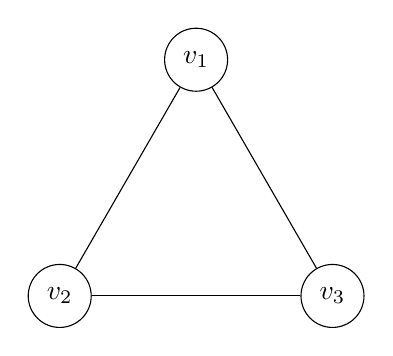
\begin{tikzpicture}[every node/.style={circle, draw, minimum size=8mm}]
        \node (v1) at (90:2) {$v_1$};
        \node (v2) at (210:2) {$v_2$};
        \node (v3) at (330:2) {$v_3$};

        \draw (v1) -- (v2);
        \draw (v2) -- (v3);
        \draw (v3) -- (v1);
    \end{tikzpicture}
    \]
\end{example}
\begin{definition}{Variables and Free variables}
    Variables in a term is defined as:
    \begin{align*}
        &Var(x) = x\\
        &Var(c) = \emptyset\\
        &Var(f(t_1, \dots, t_k)) = \bigcup_1^k Var(t_i)
    \end{align*}
    Free variables in a formula can be defined as:
    \[FVar(\forall x, \phi) = FVar(\phi) \setminus \{x\}\]
    \[FVar(\exists x, \phi) = FVar(\phi) \setminus \{x\}\]
    In words, free variables are variables apppear in a formula that are not bounded by quantifers
\end{definition}


\begin{definition}{Satisfaction of FOL formula} 
    \[\phi \text{ is satisfiable} \iff \exists (\mathfrak{A}, \alpha),  \mathfrak{A}, \alpha\models \phi\]
\end{definition}

\begin{definition}{Logical Consequence}
    \[\Gamma \models \phi \iff \forall (\mathfrak{A}, \alpha), \mathfrak{A}, \alpha \models \Gamma \implies \mathfrak{A}, \alpha \models \phi\]
\end{definition}

\begin{lemma}[Relevance Lemma for FOL]
    Let $\phi$ be a FOL formula, let $\mathfrak{A}$ be a structure and let $\alpha_1,\alpha_2$ be
    variable assignments such that for all $x \in FVar(\phi)$,
    \[
    \alpha_1(x) = \alpha_2(x).
    \]
    Then
    \[
    \mathfrak{A},\alpha_1 \models \phi \iff \mathfrak{A},\alpha_2 \models \phi.
    \]
    \end{lemma}
    
    \begin{proof}
        By symmetry, we only need to prove if for all $x\in FVar(\phi), \alpha_1(x) = \alpha_2(x)$
        then
        \[
    \mathfrak{A},\alpha_1 \models \phi \implies \mathfrak{A},\alpha_2 \models \phi.
    \]
    \begin{lemma}[Substitution lemma]
        \[
        \mathfrak{A}, \alpha \models \phi[x \mapsto t] \iff \mathfrak{A}, \alpha[x \mapsto Val_{\mathfrak{A}, \alpha}(t)] \models \phi
        \]        
    \end{lemma}
    \begin{lemma}[Substitution lemma]
        \[\forall x \in Var(t), \alpha_1(x) = \alpha_2(x) \implies Val_{\mathfrak{A}, \alpha_1}(t) = Val_{\mathfrak{A}, \alpha_2}(t)\]
    \end{lemma}\begin{lemma}[Substitution lemma]
        \[\mathfrak{A}\models \psi[x \mapsto t] \iff \mathfrak{A}, \alpha[x \mapsto Val_{\mathfrak{A}(t)}] \models \psi\]
    \end{lemma}
    \begin{lemma}
        \[Val_{\mathfrak{A}, \alpha}(t[x\mapsto t']) = Val_{\mathfrak{A}, \alpha[x \mapsto Val_{\mathfrak{A}, \alpha}(t')]}(t)\]
    \end{lemma}
    \begin{proof}
    \subsubsection*{Base case: }
    \begin{enumerate}
        \item $t = c \in C$: 
        \[Val_{\mathfrak{A}, \alpha}(t[x \mapsto t']) = Val_{\mathfrak{A}, \alpha}(c) = I(c)\]
        \[Val_{\mathfrak{A}, \alpha[x \mapsto Val_{\mathfrak{A}, \alpha}(t')]}(t) = Val_{\mathfrak{A}, \alpha[x \mapsto Val_{\mathfrak{A}, \alpha}(t')]}(c) = I(c)\]
        \item $t = y \in V$:\\
        Case 1: $x = y$
        \[
        \implies y[x \mapsto t'] = t'
        \]
        \[
        Val_{\mathfrak{A}, \alpha}(y[x \mapsto t']) = Val_{\mathfrak{A}, \alpha}(t')
        \]
        \[
        Val_{\mathfrak{A}, \alpha[x \mapsto Val_{\mathfrak{A},\alpha}(t')]}(y)
        = \alpha[x \mapsto Val_{\mathfrak{A},\alpha}(t')](y)
        = Val_{\mathfrak{A},\alpha}(t')
        \]
        Case 2: $x \neq y$
        \[
        \implies y[x \mapsto t'] = y
        \]
        \[
        Val_{\mathfrak{A}, \alpha}(y[x \mapsto t']) = Val_{\mathfrak{A}, \alpha}(y) = \alpha(y)
        \]
        \[
        Val_{\mathfrak{A}, \alpha[x \mapsto Val_{\mathfrak{A},\alpha}(t')]}(y)
        = \alpha[x \mapsto Val_{\mathfrak{A},\alpha}(t')](y)
        = \alpha(y)
        \]
    \end{enumerate}
    \subsubsection*{Inductive step: $t = f(t_1, \dots)$}
    \[
        t[x \mapsto t'] = 
        f(t_1[x \mapsto t'], t_2[x \mapsto t'], \dots)
    \]
    \[
        Val_{\mathfrak{A}, \alpha}(t[x \mapsto t']) = 
        Val_{\mathfrak{A}, \alpha}(f(t_1[x \mapsto t'], t_2[x \mapsto t'], \dots)) =
    \]
    \[
        I(f)(Val_{\mathfrak{A}, \alpha}(t_1[x \mapsto t']), Val_{\mathfrak{A}, \alpha}(t_2[x \mapsto t']), \dots)
    \]
    The other side
    \[
        Val_{\mathfrak{A}, \alpha[x \mapsto Val_{\mathfrak{A},\alpha}(t')]}(f(t_1, t_2, \dots)) = 
        I(f)(Val_{\mathfrak{A}, \alpha}(t_1[x \mapsto t']), Val_{\mathfrak{A}, \alpha}(t_2[x \mapsto t']), \dots)
    \]
    \end{proof}
    \begin{proof}
        We prove the substitution lemma for formulae by structural induction on $\psi$.
        
        \subsubsection*{Base case: $\psi \equiv t_1 = t_2$}
        \[
        \psi[x \mapsto t] \equiv t_1[x \mapsto t] = t_2[x \mapsto t]
        \]
        Thus
        \[
        \mathfrak{A}, \alpha \models \psi[x \mapsto t]
        \iff
        Val_{\mathfrak{A}, \alpha}(t_1[x \mapsto t])
        =
        Val_{\mathfrak{A}, \alpha}(t_2[x \mapsto t]).
        \]
        By the substitution lemma for terms,
        \[
        Val_{\mathfrak{A}, \alpha}(t_1[x \mapsto t])
        =
        Val_{\mathfrak{A}, \alpha[x \mapsto Val_{\mathfrak{A}, \alpha}(t)]}(t_1)
        \]
        and
        \[
        Val_{\mathfrak{A}, \alpha}(t_2[x \mapsto t])
        =
        Val_{\mathfrak{A}, \alpha[x \mapsto Val_{\mathfrak{A}, \alpha}(t)]}(t_2).
        \]
        Hence
        \[
        Val_{\mathfrak{A}, \alpha[x \mapsto Val_{\mathfrak{A}, \alpha}(t)]}(t_1)
        =
        Val_{\mathfrak{A}, \alpha[x \mapsto Val_{\mathfrak{A}, \alpha}(t)]}(t_2),
        \]
        that is,
        \[
        \mathfrak{A}, \alpha[x \mapsto Val_{\mathfrak{A}, \alpha}(t)] \models t_1 = t_2.
        \]
        
        \subsubsection*{Inductive steps}
        \begin{enumerate}
            \item $\psi \equiv R(t_1, \dots, t_n)$.
        
            \[
            \psi[x \mapsto t] \equiv R(t_1[x \mapsto t], \dots, t_n[x \mapsto t]).
            \]
            Then
            \[
            \mathfrak{A}, \alpha \models \psi[x \mapsto t]
            \iff
            \bigl(Val_{\mathfrak{A}, \alpha}(t_1[x \mapsto t]), \dots, Val_{\mathfrak{A}, \alpha}(t_n[x \mapsto t])\bigr) \in I(R).
            \]
            By the substitution lemma for terms, for each $i$,
            \[
            Val_{\mathfrak{A}, \alpha}(t_i[x \mapsto t])
            =
            Val_{\mathfrak{A}, \alpha[x \mapsto Val_{\mathfrak{A}, \alpha}(t)]}(t_i).
            \]
            \[
            \bigl(Val_{\mathfrak{A}, \alpha[x \mapsto Val_{\mathfrak{A}, \alpha}(t)]}(t_1), \dots,
            Val_{\mathfrak{A}, \alpha[x \mapsto Val_{\mathfrak{A}, \alpha}(t)]}(t_n)\bigr) \in I(R),
            \]
            \[
            \mathfrak{A}, \alpha[x \mapsto Val_{\mathfrak{A}, \alpha}(t)] \models R(t_1, \dots, t_n).
            \]
        
            \item $\psi \equiv \neg \phi$.
        
            \[
            \mathfrak{A}, \alpha \models (\neg \phi)[x \mapsto t]
            \iff
            \mathfrak{A}, \alpha \models \neg (\phi[x \mapsto t])
            \]
            \[
            \iff
            \mathfrak{A}, \alpha \not\models \phi[x \mapsto t].
            \]
            By IH,
            \[
            \mathfrak{A}, \alpha \models \phi[x \mapsto t]
            \iff
            \mathfrak{A}, \alpha[x \mapsto Val_{\mathfrak{A}, \alpha}(t)] \models \phi.
            \]
            \[
            \mathfrak{A}, \alpha[x \mapsto Val_{\mathfrak{A}, \alpha}(t)] \not\models \phi,
            \]
            \[
            \mathfrak{A}, \alpha[x \mapsto Val_{\mathfrak{A}, \alpha}(t)] \models \neg \phi.
            \]
        
            \item $\psi \equiv \phi_1 \lor \phi_2$.
        
            \[
            \mathfrak{A}, \alpha \models (\phi_1 \lor \phi_2)[x \mapsto t]
            \iff
            \mathfrak{A}, \alpha \models \phi_1[x \mapsto t] \lor \phi_2[x \mapsto t].
            \]
            \[
            \mathfrak{A}, \alpha \models \phi_1[x \mapsto t]
            \quad \text{or} \quad
            \mathfrak{A}, \alpha \models \phi_2[x \mapsto t].
            \]
            By IH
            \[
            \mathfrak{A}, \alpha[x \mapsto Val_{\mathfrak{A}, \alpha}(t)] \models \phi_1
            \quad \text{or} \quad
            \mathfrak{A}, \alpha[x \mapsto Val_{\mathfrak{A}, \alpha}(t)] \models \phi_2.
            \]
            \[
            \mathfrak{A}, \alpha[x \mapsto Val_{\mathfrak{A}, \alpha}(t)] \models \phi_1 \lor \phi_2.
            \]
        \end{enumerate}
        \end{proof}
    \end{proof}
\begin{lemma}[Analogous relevance lemma on structure]
    If $\mathfrak{A}$ and $\mathfrak{B}$ agree on all parameters ocucr in $\phi$, then $\mathfrak{A} \models \phi \iff \mathfrak{B} \models \phi$\\
    If 
    \begin{align*}
        &\forall c \in C, Val_{\mathfrak{A}, \alpha}(c) = Val_{\mathfrak{B}, \alpha}(c)\\
        &\forall x \in V, Val_{\mathfrak{A}, \alpha}(x) = Val_{\mathfrak{B}, \alpha}(x)\\
        &\forall f(t, \dots), Val_{\mathfrak{A}, \alpha}(f(t, \dots)) = Val_{\mathfrak{B}, \alpha}(f(t, \dots))\\
        &\forall R(t, \dots), R(t, \dots) \in I_{\mathfrak{A}}(R) \iff R(t, \dots) \in I_{\mathfrak{B}}(R)
    \end{align*}
    \[\mathfrak{A} \models \phi \iff \mathfrak{B} \models \phi\]
\end{lemma}
\section{Compactness of First Order Logics}
\begin{definition}{Compactness Theorem for First Order Logics}
\[\Gamma \text{ is satisfiable } \iff \Gamma \text{ is finitely satisfiable }\]
\[\Gamma \text{ is satisfiable } \iff \forall \Gamma' \subseteq_{fin} \Gamma, \exists (\mathfrak{A}, \alpha), \mathfrak{A}, \alpha \models \Gamma'\]
\end{definition}
\begin{theorem}
    Structures are not countable, and the uncountability is uncapped, as $U$ and $I$ can be arbitrarily defined
\end{theorem}
\begin{definition}{Prenex Normal Form}
    $\phi$ is in Prenex Normal Form if all quantifiers are in the beginning of the formula. 
    \[\phi \equiv Q_1x_1Q_2x_2\dots\psi\]
    Where $\psi$ is the matrix of $\phi$, which is a quantifier-free formula.
\end{definition}
\subsection{Prenex Normal Form}
\begin{enumerate}
    \item \textbf{Remove implication and biconditional.}

    Replace
    \[
    A \rightarrow B \equiv \neg A \lor B
    \]
    \[
    A \leftrightarrow B \equiv (A \rightarrow B) \land (B \rightarrow A)
    \]

    \item \textbf{Push negations inward (Negation Normal Form).}

    Apply De Morgan's laws and quantifier negation:
    \[
    \neg(A \land B) \equiv \neg A \lor \neg B
    \]
    \[
    \neg(A \lor B) \equiv \neg A \land \neg B
    \]
    \[
    \neg \forall x \, \varphi \equiv \exists x \, \neg \varphi
    \]
    \[
    \neg \exists x \, \varphi \equiv \forall x \, \neg \varphi
    \]

    After this step, negations appear only directly in front of atomic formulas.

    \item \textbf{Standardize variables apart: $\alpha$-renaming}

    Rename bound variables so that each quantifier binds a unique variable and no variable is bound by more than one quantifier.

    \item \textbf{Move quantifiers outward.}

    Move quantifiers across logical connectives when the variable does not occur free in the other formula. For example,
    \[
    (\forall x \, A) \land B \equiv \forall x (A \land B)
    \quad \text{if } x \notin \mathrm{FV}(B)
    \]
    \[
    (\exists x \, A) \lor B \equiv \exists x (A \lor B)
    \quad \text{if } x \notin \mathrm{FV}(B)
    \]

    Continue moving quantifiers outward until all quantifiers appear at the front of the formula.

    \item \textbf{Obtain Prenex Normal Form.}

    The formula now has the form
    \[
    Q_1 x_1 \; Q_2 x_2 \; \dots \; Q_n x_n \; \varphi
    \]
    where each \(Q_i \in \{\forall,\exists\}\) and \(\varphi\) is quantifier-free.
\end{enumerate}
\begin{example}
    \[\phi \equiv P(x) \land \forall z (R(x, z)\lor \exists y Q(y))\]
    \begin{enumerate}
        \item move out quantifiers: 
        \[\phi \equiv P(x) \land \forall z\exists y (R(x, z) \lor Q(y))\]
        \[\phi \equiv \forall z\exists y [P(x) \land (R(x, z) \lor Q(y))]\]
        \item PNF obtained, $\varphi \equiv P(x) \land (R(x, z) \lor Q(y))$
    \end{enumerate}
\end{example}
\begin{example}
    \[\phi \equiv \forall x (\neg P(x) \lor \exists y (Q(x, y) \land \forall z R(y, z))) \lor \exists x S(x)\]
    \begin{enumerate}
        \item $\alpha$-renaming
        \[\phi \equiv \forall x (\neg P(x) \lor \exists y (Q(x, y) \land \forall z R(y, z))) \lor \exists u S(u)\]
        \item 
    \end{enumerate}
\end{example}
\begin{lemma}
    $\psi$, the PNF of $\phi$ is logically equivalent to $\phi$
    \[\forall (\mathfrak{A}, \alpha), \mathfrak{A}, \alpha \models \psi \iff \mathfrak{A}, \alpha \models \phi\]
\end{lemma}
\begin{proof}
    
\end{proof}
\begin{definition}{Universally quantified formula}
$\phi$ is universally wuantified if all quantifiers in $\phi$ are $\forall$. Analogous to Existantial quantified formula    
\end{definition}
\begin{definition}{Sentence}
    $\phi$ is a sentence if there is no free variables. 
    \[FVar(\phi) = \emptyset\]
\end{definition}
To determine satisfiability, we can ignore existential quantifiers. 
\begin{theorem}
    Let $\varphi$ be a formula and $FVar(\varphi) = \{x_1, x_2, \dots, x_k\} \varphi$ is satisfiable iff 
    \[\varphi' \equiv \exists x_1 \exists x_2, \dots, \exists x_k \varphi \text{ is satisfiable}\]
    $\varphi'$ is a sentence
\end{theorem}

\begin{definition}{Skolemization}
    Transform PNF into universally quantified PNF. \\
    $\forall \phi, \exists \phi'$, such that
    \begin{enumerate}
        \item $\phi$ and $\phi'$ are equisatisfiable. (Not necessarily equivalent!)
        \item $\phi'$ is universally quantified PNF
    \end{enumerate}
\end{definition}
\subsection{Skolemization}
\begin{enumerate}
    \item \textbf{Convert the formula to prenex normal form.}

    Transform the formula so that all quantifiers appear at the front:
    \[
    Q_1 x_1 \; Q_2 x_2 \; \dots \; Q_n x_n \; \varphi
    \]
    where \(\varphi\) is quantifier-free.

    \item \textbf{Process quantifiers from left to right.}

    For each existential quantifier \(\exists x\), determine the universal
    variables that precede it in the prefix.

    \item \textbf{Replace existential variables with Skolem terms.}

    \begin{itemize}
        \item If \(\exists x\) has no preceding universal quantifiers,
        replace \(x\) with a new Skolem constant \(c\).
        \[
        \exists x \, P(x) \;\;\Rightarrow\;\; P(c)
        \]

        \item If \(\exists x\) is preceded by universal variables
        \(u_1,\dots,u_k\), replace \(x\) with a new Skolem function
        \(f(u_1,\dots,u_k)\).
        \[
        \forall u_1 \dots \forall u_k \exists x \, P(x,u_1,\dots,u_k)
        \;\Rightarrow\;
        P(f(u_1,\dots,u_k),u_1,\dots,u_k)
        \]
    \end{itemize}

    \item \textbf{Remove the existential quantifier.}

    After substitution with the Skolem term, delete the corresponding
    existential quantifier from the prefix.

    \item \textbf{Repeat until no existential quantifiers remain.}

    The resulting formula contains only universal quantifiers.

    \item \textbf{Optionally drop universal quantifiers.}

    In many applications (e.g., resolution), the remaining universal
    quantifiers are omitted, since variables are implicitly assumed to
    be universally quantified.
\end{enumerate}
\begin{example}
    \[\phi \equiv \exists x P(x) \land \forall z(R(x, z) \lor \exists y Q(y))\]
    \begin{enumerate}
        \item convert to PNF
        \[\phi \equiv \exists x \forall z \exists y (P(x) \land (R(x, z) \lor Q(y)))\]
        \item if the leftmost quantifier is exisitential, replace the variable with a new constant $c$
        \[\phi' \equiv \forall z \exists y (P(c_x) \land (R(c_x, z) \lor Q(y)))\]
        \[c_x \notin \Sigma\]
        At this stage, $\phi$ and $\phi'$ are equisatisfiable. No longer equivalent
        \begin{proof}
            $\phi$ is satisfiabe $\implies \exists \mathfrak{A}, \alpha \models \phi$. We can construct a new signature and structure from it as such
            \[\Sigma' = \Sigma \cup \{c_x\}, \quad I'(c_x) = \alpha(x)\]
            We can show that $\mathfrak{A}', \alpha \models \phi'$\\
            The other way can be done similarly
        \end{proof}
        \item if the next existential quantifie is not the outer most, add a new funciton symbol to replace each variable quantified by the existential
        quantifer with the function call using all previous universally quantified variables
        \[\phi'' \equiv \forall z (P(c_x)) \land (R(c_x, z)\lor Q(f_y(z))) \]
        We can show that $\phi'$ and $\phi''$ are equisatisfiable
    \end{enumerate}
\end{example}

\begin{theorem}
    Skolemization preserves satisfiability.
\end{theorem}

\begin{proof}
    Consider skolemization as a recursive algorithm described as follows:\\
\begin{algorithm}[H]
    \caption{Skolemization on Prenex Formula}
    \KwIn{
    Signature $\Sigma = (C, F, R)$; \\
    Formula $\phi = (\pi, \psi)$ where $\pi$ is a quantifier prefix and $\psi$ is quantifier-free\;
    List $u$ of universally quantified variables in scope (initially empty).
    }
    \KwOut{
    Skolemized formula $(\pi', \psi')$ equisatisfiable with $\phi$.
    }
    
    \If{$\pi$ is empty}{
        \Return$(\emptyset, \psi)$
    }
    
    $(q, x) \gets \text{head}(\pi)$\;
    $\pi_{\text{rest}} \gets \text{tail}(\pi)$
    
    \If{$q = \exists$}{
        \eIf{$u$ is empty}{
            introduce fresh constant $c_x$\;
            $\Sigma.C \gets \Sigma.C \uplus \{c_x\}$\;
            \Return{Skol$(\Sigma, (\pi_{\text{rest}}, \psi[x \mapsto c_x]), u)$}
        }{
            introduce fresh function $f_x$ of arity $|u|$\;
            $\Sigma.F \gets \Sigma.F \uplus \{f_x\}$\;
            let $t = f_x(u_1, \dots, u_k)$ where $u = [u_1, \dots, u_k]$\;
            \Return{Skol$(\Sigma, (\pi_{\text{rest}}, \psi[x \mapsto t]), u)$}
        }
    }
    \Else{ \tcp{$q = \forall$}
        $u' \gets u \cdot x$ \tcp{append $x$ to $u$}
        $(\pi', \psi') \gets$ Skol$(\Sigma, (\pi_{\text{rest}}, \psi), u')$\;
        \Return{$((\forall x)\cdot \pi', \psi')$}
    }
\end{algorithm}
We claim that the invariant is the satisfiability of input and output is the same.
Let $\text{Skol}(\Sigma, (\pi, \psi), u)$ be the recursive algorithm defined. 
We prove by induction on the length of the quantifier prefix $n = |\pi|$ that the algorithm preserves equisatisfiability.

\subsection*{Inductive Hypothesis (IH)}
For any prefix $\pi$ of length $n$, any signature $\Sigma$, and any list of universal variables $u = [u_1, \dots, u_k]$, 
a formula $\phi = \forall u (\pi \psi)$ is satisfiable in a $\Sigma$-structure $\mathfrak{A}$ 
if and only if there exists a larger $\mathfrak{A}'$ than $\mathfrak{A}$ to $\Sigma'$ (containing new symbols) 
such that $\mathcal{A}'$ satisfies the output of $\text{Skol}(\Sigma, (\pi, \psi), u)$.
\[\mathfrak{A} \models \phi = \forall u (\pi \psi) \iff \mathfrak{A}' \models {Skol}(\Sigma, (\pi, \psi), u)\]

\subsection*{Case 1: Base Case ($n = 0$)}
If $\pi$ is empty, the algorithm returns $(\emptyset, \psi)$, trivially equisatisfiable

\subsection*{Case 2: Universal Case ($q = \forall$)}
Let $\pi = \forall x \cdot \pi_{\text{rest}}$. The algorithm sets $u' = u \cdot x$ and recurses\\
We will show that:
$$\mathfrak{A} \models \forall u \forall x (\pi_{\text{rest}} \psi) \iff \mathfrak{A}' \models \forall u \forall x ({Skol}(\pi_{\text{rest}}, \psi, u'))$$

\begin{itemize}
    \item \textbf{ ($\Rightarrow$):} Suppose $\mathfrak{A} \models \forall u \forall x (\pi_{\text{rest}} \psi)\implies \mathfrak{A} \models \forall (u \cup \{x\}) (\pi_{\text{rest}} \psi)$. 
    There exists an expansion $\mathfrak{A}'$ such that $\mathfrak{A}' \models \forall (u \cup \{x\}) {Skol}(\pi_{\text{rest}}, \psi, u')$. rearrange the quantifiers gives $\mathfrak{A}' \models \forall u \forall x {Skol}(\dots)$.
    \item \textbf{ ($\Leftarrow$):} Suppose $\mathfrak{A}' \models {Skol}(\pi_{\text{rest}}, \psi, u')$. Since $\mathfrak{A}'$ is an expansion of $\mathfrak{A}$, and the universal quantifier $\forall x$ 
    does not introduce new symbols in this step, same logic 
\end{itemize}

\subsection*{Case 3: Existential Case ($q = \exists$)}

\end{proof}
\begin{theorem}[Herbrand's Theorem]
    Informally, if a first-order formula $\phi$ is satisfiable, then its
    satisfiability is witnessed by a special kind of structure called a
    \emph{Herbrand structure}.
    \end{theorem}
    
    \begin{definition}[Herbrand structure]
    Let $\Sigma = (\mathcal{C}, \mathcal{F}, \mathcal{P})$ be a signature.
    A structure
    \[
    \mathfrak{A} = (U, I)
    \]
    is a \emph{Herbrand structure} if
    
    \begin{enumerate}
        \item The universe is the \emph{Herbrand universe}
        \[
        U = T_{\mathcal{C} \cup \mathcal{F}},
        \]
        the set of all ground terms constructed from the constant symbols
        $\mathcal{C}$ and function symbols $\mathcal{F}$.
    
        \item The interpretation $I$ is fixed syntactically:
        \begin{itemize}
            \item For every constant symbol $c \in \mathcal{C}$,
            \[
            I(c) = c
            \]
    
            \item For every function symbol $f \in \mathcal{F}$ of arity $n$,
            \[
            I(f)(t_1,\dots,t_n) = f(t_1,\dots,t_n)
            \]
        \end{itemize}
    \end{enumerate}
    \end{definition}


\begin{definition}{Ground term}
    \[gt := c \mid f(gt, \dots)\]
    Basically terms without variables
\end{definition}
\begin{definition}{Ground Atom (Let's ignore = first)}
    \[ga := R(gt, \dots)\]
\end{definition}
\begin{definition}[Ground Formula]
    \[gf := gt = gt \mid R(gt, \dots) \mid \neg gf \mid gf \lor gf\]
    No variables, no quantifiers
\end{definition}
Now that we have developed the machinery needed to prove Compactness for first-order logic, we outline the overall proof strategy.
From the definition of grounding, it is clear that the goal is to connect first-order logic with propositional logic. 
By grounding, we eliminate variables and quantifiers, and treat each ground atom as a propositional atom. In this way, we translate the satisfiability problem for a first-order theory into a corresponding satisfiability problem in propositional logic.
This suggests the following proof plan: establish a correspondence between satisfiability and finite satisfiability for $\Gamma$ and for its grounding $\mathrm{Gr}(\Gamma)$, then apply Compactness of propositional logic to $\mathrm{Gr}(\Gamma)$ in order to deduce Compactness for first-order logic.
\[
\begin{tikzcd}[column sep=8em, row sep=4em]
\Gamma \text{ is satisfiable}
    \arrow[r, dashed, shift left=0.6ex]
    \arrow[d, shift left=0.6ex, "\text{(1)}"]
&
\Gamma \text{ is finitely satisfiable}
    \arrow[l, dashed, shift left=0.6ex]
    \arrow[d, shift left=0.6ex, "\text{(3)}"]
\\
\mathrm{Gr}(\Gamma) \text{ is propositionally satisfiable}
    \arrow[u, shift left=0.6ex, "\text{(2)}"]
    \arrow[r, leftrightarrow, left=0.6ex, "\text{Compactness of PL}"]
&
\mathrm{Gr}(\Gamma) \text{ is finitely satisfiable}
    \arrow[u, shift left=0.6ex, "\text{(4)}"]
\end{tikzcd}
\]

\begin{definition}[Ground instantiation]
    $\phi$ is a universally quantified sentence in PNF, let $\psi$ be a ground formula, with the same signature. $\psi$ is a ground instantiation of $\phi$, or $Gr(\phi) = \psi$ if:
    \[\phi = \forall x_1\forall x_2, \dots, \forall x_n \cdot \gamma\]
    There are n ground terms $gt_1, gt_2, \dots, gt_n$, such that 
    \[\psi = \gamma[x_1 \mapsto gt_1][x_2 \mapsto gt_2]\dots[x_n \mapsto gt_n]\]
\end{definition}
\begin{definition}[Ground instantiation of a set]
    \[Gr(\Gamma) = \bigcup_{\phi\in \Gamma} Gr(\phi)\]
\end{definition}
\begin{lemma}[Ground instantiation of a formula is countable]
\end{lemma}
\begin{corollary}[Ground instantiation of a set is countable]
\end{corollary}
\begin{definition}[Ground valuation]
    \[gv: ga_\Sigma \mapsto \{true, false\}\]
    \begin{align*}
        &gv \models_{gr} R(t, \dots) \iff gv(R(t, \dots)) = true\\
        &gv \models_{gr} \neg gf \iff gv \not\models_{gr} gf\\
        &gv \models_{gr} gf_1 \lor gf_2 \iff gv \models_{gr} gf_1 \text{ OR } gv \models_{gr} gf_2\\
    \end{align*}
\end{definition}




\begin{definition}[Propositionally satisfiable]
    A ground formula $gf$ is propositionally satisfiable if 
    \[\exists \tau \models_{gr} gf\]
\end{definition}
\begin{definition}[Propositionally satisfiable set]
    A set of grounf formula $\Gamma$ is propositionally satisfiable if there exist a ground atomic valuation $\tau$
    such that 
    \[\forall \phi \in \Gamma, \tau \models_{Gr} \phi\]
    
\end{definition}

\subsection{Proof of the compactness theorem for FOL}
Let's first consider the case without equality, the definition of ground formula becomes: 
\[gf := R(ga, \dots) \mid \neg gf \mid gf \lor gf\]
\subsubsection{$\Gamma$ is satisfiable $\implies Gr(\Gamma)$ is propositionally satisfiable}



\begin{lemma}[Substitution Lemma for Ground Terms]
    Let $\mathfrak A = (U,I)$ be a structure, $\psi$ a formula, $x$ a variable, and $t$ a ground term. Then for any assignment $\alpha$,
    \[
    \mathfrak A, \alpha \models \psi[x \mapsto t]
    \;\Longleftrightarrow\;
    \mathfrak A, \alpha[x \mapsto \operatorname{Val}_{\mathfrak A}(t)] \models \psi.
    \]
    \end{lemma}
    \begin{proof}
        We have proven a more general case of substitution for FOL formula and terms
    \end{proof}
    
    \begin{lemma}[Ground Instantiation for Universal Prefix]
    Let $\mathfrak A = (U,I)$ be a structure and
    \[
    \phi = \forall x_1 \cdots \forall x_n\,\psi.
    \]
    If $\mathfrak A \models \phi$, then for all ground terms $t_1,\dots,t_n$,
    \[
    \mathfrak A \models \psi[x_1 \mapsto t_1]\dots[x_n \mapsto t_n].
    \]
    \end{lemma}
    \begin{proof}
        Assume $\mathfrak A \models \forall x_1 \cdots \forall x_n\,\psi$.
        
        Let $t_1,\dots,t_n$ be arbitrary ground terms. Define
        \[
        u_i = \operatorname{Val}_{\mathfrak A}(t_i) \in U \quad (1 \le i \le n).
        \]
        
        By the semantics of universal quantifiers,
        \[
        \mathfrak A \models \forall x_1 \cdots \forall x_n\,\psi
        \;\Longrightarrow\;
        \mathfrak A, \alpha[x_1 \mapsto u_1]\cdots[x_n \mapsto u_n] \models \psi
        \]
        for every assignment $\alpha$.
        
        By the substitution lemma for ground terms,
        \[
        \mathfrak A, \alpha \models \psi[x_1 \mapsto t_1]\cdots[x_n \mapsto t_n]
        \;\Longleftrightarrow\;
        \mathfrak A, \alpha[x_1 \mapsto u_1]\cdots[x_n \mapsto u_n] \models \psi.
        \]
        
        Hence,
        \[
        \mathfrak A, \alpha \models \psi[x_1 \mapsto t_1]\cdots[x_n \mapsto t_n].
        \]
        
        Since $\alpha$ was arbitrary,
        \[
        \mathfrak A \models \psi[x_1 \mapsto t_1]\cdots[x_n \mapsto t_n].
        \]
        \end{proof}
        \begin{lemma}[Ground Semantic Equivalence] Let $\mathfrak A = (U,I)$ and $\tau$ be defined as above. Then for every ground formula $\chi$, \[ \mathfrak A \models \chi \;\Longleftrightarrow\; \tau \models_{Gr} \chi. \] \end{lemma}
        \begin{proof}
            Trivial by definition
        \end{proof}

    \begin{lemma}[Ground Semantic Equivalence]
    Let $\mathfrak A = (U,I)$ and $\tau$ be defined as above. Then for every ground formula $\chi$,
    \[
    \mathfrak A \models \chi
    \;\Longleftrightarrow\;
    \tau \models_{Gr} \chi.
    \]
    \end{lemma}
    \begin{proof}
        We prove the claim by structural induction on the ground formula $\chi$.
        
        \textbf{Base case:} $\chi$ is a ground atom. Then
        \[
        \mathfrak A \models \chi
        \;\Longleftrightarrow\;
        \tau \models_{Gr} \chi
        \]
        by the Atomic Agreement Lemma.
        
        \textbf{Inductive case 1:} $\chi = \neg \chi_1$ for some ground formula $\chi_1$.
        
        By the semantics of negation,
        \[
        \mathfrak A \models \neg \chi_1
        \;\Longleftrightarrow\;
        \mathfrak A \not\models \chi_1.
        \]
        By the induction hypothesis,
        \[
        \mathfrak A \not\models \chi_1
        \;\Longleftrightarrow\;
        \tau \not\models_{Gr} \chi_1.
        \]
        Again by the semantics of negation,
        \[
        \tau \not\models_{Gr} \chi_1
        \;\Longleftrightarrow\;
        \tau \models_{Gr} \neg \chi_1.
        \]
        Hence
        \[
        \mathfrak A \models \neg \chi_1
        \;\Longleftrightarrow\;
        \tau \models_{Gr} \neg \chi_1.
        \]
        
        \textbf{Inductive case 2:} $\chi = \chi_1 \vee \chi_2$ for some ground formulas $\chi_1,\chi_2$.
        
        By the semantics of disjunction,
        \[
        \mathfrak A \models \chi_1 \vee \chi_2
        \;\Longleftrightarrow\;
        (\mathfrak A \models \chi_1 \text{ or } \mathfrak A \models \chi_2).
        \]
        By the induction hypothesis,
        \[
        (\mathfrak A \models \chi_1 \text{ or } \mathfrak A \models \chi_2)
        \;\Longleftrightarrow\;
        (\tau \models_{Gr} \chi_1 \text{ or } \tau \models_{Gr} \chi_2).
        \]
        Again by the semantics of disjunction,
        \[
        (\tau \models_{Gr} \chi_1 \text{ or } \tau \models_{Gr} \chi_2)
        \;\Longleftrightarrow\;
        \tau \models_{Gr} \chi_1 \vee \chi_2.
        \]
        Hence
        \[
        \mathfrak A \models \chi_1 \vee \chi_2
        \;\Longleftrightarrow\;
        \tau \models_{Gr} \chi_1 \vee \chi_2.
        \]
        
        Therefore, for every ground formula $\chi$,
        \[
        \mathfrak A \models \chi
        \;\Longleftrightarrow\;
        \tau \models_{Gr} \chi.
        \]
        \end{proof}
    
    \begin{lemma}[Grounding Preserves Truth]
    Let $\Gamma$ be a set of sentences (in Skolem form). If
    \[
    \mathfrak A \models \Gamma,
    \]
    then
    \[
    \mathfrak A \models Ground(\Gamma).
    \]
    \end{lemma}
    
    \begin{lemma}[Transfer to Ground Valuation]
    Let $\mathfrak A = (U,I)$ and $\tau$ be defined as above. If
    \[
    \mathfrak A \models Ground(\Gamma),
    \]
    then
    \[
    \tau \models_{Gr} Ground(\Gamma).
    \]
    \end{lemma}






\begin{proof}
    $\Gamma$ is satisfiable $\implies$ there exists a strucutre $\mathfrak{A}$ such that
    \[\mathfrak{A} \models \Gamma\]
    Define ground valuation on atoms 
    \[\tau: ga_{\Sigma} \mapsto \{true, false\}\]
    and for all ground atoms over $\Sigma$, define
    \[\tau(a) = true \iff \mathfrak{A} \models a\]
    Now we will show that: $\mathfrak{A} \models \phi \implies \tau \models_{Gr} \phi$\\
    Define ground valuation $\tau$ as such:
    \[\tau(R(t_1, \dots t_n)) = \begin{cases}
        true \quad \text{if } (Val_{\mathfrak{A}}(t_1), \dots, Val_{\mathfrak{A}}(t_n))\in I_{\mathfrak{A}}(R)\\
        false \quad \text{ otherwise}
    \end{cases}\]
    \subsubsection*{Base case: $\phi$ is ground atom}
    By definition, trivial
    \subsubsection*{Inductive steps: induction over the structure of formula(not gf)}
    \begin{itemize}
        \item $\varphi = \neg \phi$: $\mathfrak{A} \models \neg\phi \implies \mathfrak{A} \not\models \phi $. 
        
        \item $\varphi = \phi_1 \lor \phi_2$
    \end{itemize}

\end{proof}


\subsection{Special FOL fragments}
\subsubsection{Quantifier-free FOL}
\begin{definition}[quantifier free formula]
    \[\phi := t = t \mid R(t, \dots) \mid \neg \phi \mid \phi \lor \phi\]
    All variables are free
\end{definition}
\begin{definition}[QT-free SAT]
    QT-F SAT = $\{\phi \mid \phi \text{ is quantifier free}, \phi \text{ is satisfiable}\}$
\end{definition}
\begin{definition}[Small Model Property]
    A fragment $\mathbb{F}$ of logic is said to have the \textbf{Small Model Property} (SMP) if there exists a computable function $b_{\mathbb{F}}: \mathbb{F} \to \mathbb{N}$ such that for every formula $\phi \in \mathbb{F}$:
    \[ \text{If } \phi \text{ is satisfiable, then } \exists \mathfrak{A} \models \phi \text{ such that } |U_{\mathfrak{A}}| \leq b_{\mathbb{F}}(\phi) \]
\end{definition}
We are interested in QT-free formula because it satify the SMP
\begin{theorem}
    If $\mathbb{F}$ satisfy SM, the satiefiability of $\mathbb{F}$ is decidable.
\end{theorem}
\begin{corollary}
    $FORM_{FOL}$ does not have SMP
\end{corollary}
\begin{proof}[counter example]
    Consider the folowing formula:
    \[\phi \equiv \forall x , S(x) \neq 0 \land (x \neq y \rightarrow S(x) \neq S(y))\]
    This basically describes a structure that has no right endpoint, and no 2 unique elements have the same successor. This requires an infinite (unbounded) structure, thus $FORM_{FOL}$ does not possess the SMP
\end{proof}


\begin{proof}
    Notie that, for quantifier free formula, the set of ground insitantiateions is finite. 
    \[\phi \in QT-free SAT \iff skol(\phi) \in QT-free SAT \land \phi \text{ is grounded}\]
    As skolemization preserves satisfiability 
\end{proof}











\subsection{Homomorphism and Isomorphism}
\begin{definition}[Homomorphism]
    Let $\Sigma = (C, F, R)$ be a First order signature. $\mathfrak{A}_1 = (U_1, I_1)$ and $\mathfrak{A}_2 = (U_2, I_2)$ be $\Sigma$-structures. A function 
    \[h: U_1 \mapsto U_2\]
    is a homomorphism from $\mathfrak{A}_1$ to $\mathfrak{A}_2$ if: 
    \begin{enumerate}
        \item $\forall c \in C, h(I_1(c)) = I_2(c)$
        \item $\forall f^k \in F, \forall (u_1, \dots, u_k) \in U^k_1, h(I_1(f)(u_1, \dots, u_k)) = I_2(f)(h(u_1), \dots, h(u_k))$
        \item $\forall R^k \in R, \forall (u_1, \dots, u_k) \in U^k_1, (u_1, \dots, u_k) \in I_1(R) \iff (h(u_1), \dots, h(u_k)) \in I_2(R)$
    \end{enumerate}
\end{definition}

\begin{definition}[Isomorphism]
    Let $\Sigma = (C, F, R)$ be a First order signature. $\mathfrak{A}_1 = (U_1, I_1)$ and $\mathfrak{A}_2 = (U_2, I_2)$ be $\Sigma$-structures. A function 
    \[h: U_1 \mapsto U_2\]
    is an isomorphism from $\mathfrak{A}_1$ to $\mathfrak{A}_2$ if:  
    \begin{enumerate}
        \item $h$ is a homomorphism from $\mathfrak{A}_1$ to $\mathfrak{A}_2$
        \item $h$ is a bijection
    \end{enumerate}
    denoted as 
    \[\mathfrak{A}_1 \cong \mathfrak{A}_2\]
\end{definition}
\begin{theorem}[Isomorphism Theorem]
    \[\mathfrak{A}_1, \alpha \models \phi \iff \mathfrak{A}_2, (h \circ \alpha) \models \phi\]
\end{theorem}


\subsection{Theory}
\begin{definition}[Theory]
    A theory $T$ is a set of sentences.
\end{definition}
\begin{example}[Partial order]
    \[T_{po} = \begin{cases}
        \forall x \forall y \forall z <(x, y) \land <(y, z) \rightarrow <(x, z) \quad \text{ (transitivity)}\\
        \forall x \neg <(x, x) \quad \text{ (irreflexivity)}
    \end{cases}\]
\end{example}

\begin{definition}[T-satisfiable]
    Let $T$ be a theory over $\Sigma$, a formula $\phi$ over $\Sigma$ is T-satisfiable if 
    \[\exists \mathfrak{A}, \alpha, \mathfrak{A}, \alpha \models \phi\]
    AND
    \[\forall \psi \in T, \mathfrak{A} \models \psi\]
\end{definition}
\begin{definition}[T-validity]
    Let $T$ be a theory over $\Sigma$, a formula $\phi$ over $\Sigma$ is T-valid if 
    \[\forall \mathfrak{A}, \text{ if } \forall \psi \in T, \mathfrak{A} \models \psi \rightarrow \mathfrak{A} \models \phi\]
\end{definition}

\subsubsection{Common clauses used to define theories}
\begin{itemize}
    \item $\sigma_1 \equiv \forall x \neg(x < x) \land \forall x\forall y \forall z (x<y \land y<z \rightarrow x<z)$ (partial order)
    \item $\sigma_2 \equiv \forall x\forall y (x<y \lor x = y \lor y < x)$ (trichotomy)
    \item $\sigma_3 \equiv \forall x \forall y(x < y \rightarrow \exists z(x < z< y))$ (dense)
    \item $\sigma_4 \equiv \forall x \exists y \exists z (y < x < z)$ (no endpoints)
    \item $\varphi_1 \equiv \forall x \forall y \forall z ((x + y) + z) = x + (y + z)$ (associativity)
    \item $\varphi_2 \equiv \forall x ((x + 0 = x = 0 + x) \land (x + (-x) = (-x) + x = 0))$ (additive identity \& add. inverse axioms)
    \item $\varphi_3 \equiv \forall x \forall y (x + y = y + x)$ (commutativity)
    \item $\varphi_4 \equiv \forall x \forall y \forall z (x < y \rightarrow ((x + z) < (y + z)))$ (order-compatibility axiom for addition)
    \item $\psi_n \equiv \forall x (nx = 0 \rightarrow x = 0)$ (torsion-freeness)
\end{itemize}
Theories formed over above sentences include:
\begin{itemize}
    \item $\mathfrak{A} \models \sigma_1 \iff \mathfrak{A}$ is a partial order
    \item $\mathfrak{A} \models \{\sigma_1, \sigma_2\} \iff \mathfrak{A}$ is a linear/total order
    \item $\mathfrak{A} \models \{\sigma_1, \sigma_2, \sigma_3, \sigma_4\} \iff \mathfrak{A}$ is a dense linear order without endpoints
    \item $\mathfrak{A} \models \{\varphi_1, \varphi_2\} \iff \mathfrak{A}$ is a group
    \item $\mathfrak{A} \models \{\varphi_1, \varphi_2, \varphi_3\} \iff \mathfrak{A}$ is an abelian group
    \item $\mathfrak{A} \models \{\varphi_1, \varphi_2, \varphi_3, \varphi_4, \sigma_1, \sigma_2\} \iff \mathfrak{A}$ is an ordered abelian group
    \item $\mathfrak{A} \models \{\varphi_1, \varphi_2, \varphi_3, \psi_n\}_{n \in \mathbb{N}} \iff \mathfrak{A}$ is a torsion-free abelian group
\end{itemize}
\subsubsection{Monontonicity under theory inclusion}
\begin{lemma}
    If $T_1 \subseteq T_2$ , $\phi$ is $T_1$-valid $\implies \phi_2$ is $T_2$-valid. Or
    \[T_1 \subseteq T_2, T_1 \models \phi \implies T_2 \models \phi\]
\end{lemma}
\begin{lemma}
    If $T_1 \subseteq T_2$ , $\phi$ is $T_2$-sat $\implies \phi$ is $T_1$-sat. Or
    \[T_1 \subseteq T_2, T_2 \cup \{\phi\} \text{ is satisfiable } \implies T_1 \cup \{\phi\} \text{ is satisfiable}\]
    \[T_1 \subseteq T_2, T_1 \cup \{\phi\} \text{ is unsatisfiable } \implies T_2 \cup \{\phi\} \text{ is unsatisfiable}\]
\end{lemma}
\subsubsection{Theory of a structure}
Instead od a set of sentences, we can also define a theory with a structure. 
\begin{definition}
    Let $\mathfrak{A}$ be a structutre, 
    \[Th(\mathfrak{A}) = \{\phi \mid \phi \text{ is a sentence }, \mathfrak{A} \models \phi\}\]
\end{definition}

\begin{definition}[Class of structures]
    Let $\mathfrak{C}$ be a collection of strucutre, 
    \[Th(\mathfrak{C}) = \bigcap_{\mathfrak{A} \in \mathfrak{C}} Th(\mathfrak{A})\]
\end{definition}

\begin{definition}
    \[Th(\Gamma) = \{\phi \mid \phi \text{ is a sentence }, \Gamma \models \phi\}\]
\end{definition}

\begin{theorem}
    \[Th(Th(\Gamma)) \subseteq Th(\Gamma)\]
\end{theorem}
\begin{proof}
    Suppose otherwise, $\exists \phi \in Th(Th(\Gamma)), \phi \notin Th(\Gamma).$
    \[\phi \in Th(Th(\Gamma)) \implies Th(\Gamma) \models \phi\]
    \[\phi \notin Th(\Gamma) \implies \Gamma \not\models \phi \implies \exists \mathfrak{A}, \mathfrak{A} \models \Gamma, \mathfrak{A} \not\models \phi\]
    \[\mathfrak{A} \models Th(\Gamma), \text{ contradiction}\]
\end{proof}

\begin{theorem}
    \[Th(\Gamma) \text{ is inconsistent } \implies Th(\Gamma) \models \text{ all sentences}\]
\end{theorem}
\begin{definition}[Consistency of a theory]
    Theory $T$ is consistent if 
    \[\forall \phi, \neg (\{\phi\} \subseteq T \land \{\neg \phi \} \subseteq T)\]
\end{definition}

\begin{definition}[Completeness of a theory]
    Theory $T$ is complete if
    \[\forall \phi, \{\phi, \neg \phi\} \cap T \neq \emptyset\]
\end{definition}
\begin{lemma}
    \[Th(\mathfrak{A}) \text{ is consistnet}\]
\end{lemma}
\begin{proof}
    Suppose otherwise, $\phi, \neg \phi \in Th(\mathfrak{A}). \mathfrak{A} \models \phi \oplus \mathfrak{A} \models \neg \phi$, contradiction.
\end{proof}

\begin{lemma}
    \[Th(\mathfrak{A}) \text{ is complete}\]
\end{lemma}
\begin{proof}
    Let $\phi$ be a sentence, 
    \begin{itemize}
        \item if $\mathfrak{A} \models \phi, \phi \in Th(\mathfrak{A})$
        \item if $\mathfrak{A} \not\models \phi, \mathfrak{A} \models \neg \phi, \neg \phi \in Th(\mathfrak{A})$
    \end{itemize}
\end{proof}


\begin{lemma}
    \[Th(\mathfrak{C}) \text{ is consistent}\]
\end{lemma}

\begin{proof}
    Suppose otherwise, $\exists \phi, \phi, \neg \phi \in Th(\mathfrak{C})$
    \[\forall \mathfrak{A} \in \mathfrak{C}, \mathfrak{A} \models \phi \oplus \mathfrak{A} \models \neg \phi\]
    contradiction
\end{proof}
\begin{lemma}
    $Th(\mathfrak{C})$ is not complete.
\end{lemma}

\begin{proof}
    A theory $T$ is complete if for every sentence $\psi$, either $T \models \psi$ or $T \models \neg \psi$. To show $Th(\mathfrak{C})$ is incomplete, we can find a sentence $\phi$ such that $Th(\mathfrak{C}) \not\models \phi$ and $Th(\mathfrak{C}) \not\models \neg \phi$.
    
    Let $\phi \equiv \exists x \exists y, R(x, y)$. Consider the following two structures in $\mathfrak{C}$:

    \begin{enumerate}
        \item Structure $\mathfrak{A} = (U_{\mathfrak{A}}, I_{\mathfrak{A}})$:
        \begin{itemize}
            \item $U_{\mathfrak{A}} = \{0, 1\}$
            \item $I_{\mathfrak{A}}(R) = \{(0,1)\}$
        \end{itemize}
        In this structure, $R(0,1)$ holds, therefore $\mathfrak{A} \models \phi$. This implies $Th(\mathfrak{C}) \not\models \neg \phi$.

        \item Structure $\mathfrak{B} = (U_{\mathfrak{B}}, I_{\mathfrak{B}})$:
        \begin{itemize}
            \item $U_{\mathfrak{B}} = \{0, 1\}$
            \item $I_{\mathfrak{B}}(R) = \emptyset$
        \end{itemize}
        In this structure, no pair $(x,y)$ satisfies $R$, therefore $\mathfrak{B} \models \neg \phi$. This implies $Th(\mathfrak{C}) \not\models \phi$.
    \end{enumerate}

    Since there exists a structure in $\mathfrak{C}$ that satisfies $\phi$ and another that satisfies $\neg \phi$, the theory $Th(\mathfrak{C})$ contains neither. Thus, $Th(\mathfrak{C})$ is not complete.
\end{proof}




\begin{theorem}
    Let $T$ be a theory, $T \in RE$. 
    If $T$ is consistent and complete, $T \in REC$
\end{theorem}

\begin{proof}
    Let $E$ be an enumerator for $T$. To decide if $\psi \in T$:
    \begin{enumerate}
        \item Start $E$ to produce sentences $\sigma_1, \sigma_2, \sigma_3, \dots$
        \item For each $\sigma_i$, check if $\sigma_i = \psi$ or $\sigma_i = \neg \psi$.
        \item By completeness, one of these must eventually appear.
        \item If $\psi$ appears, accept. If $\neg \psi$ appears, reject.
    \end{enumerate}
    Since the algorithm always halts, $T \in REC$.
\end{proof}













\section{Computability}
\subsection{Halting problem}
\begin{theorem}
    The halting problem is undecidable
\end{theorem}

\begin{proof}
\[
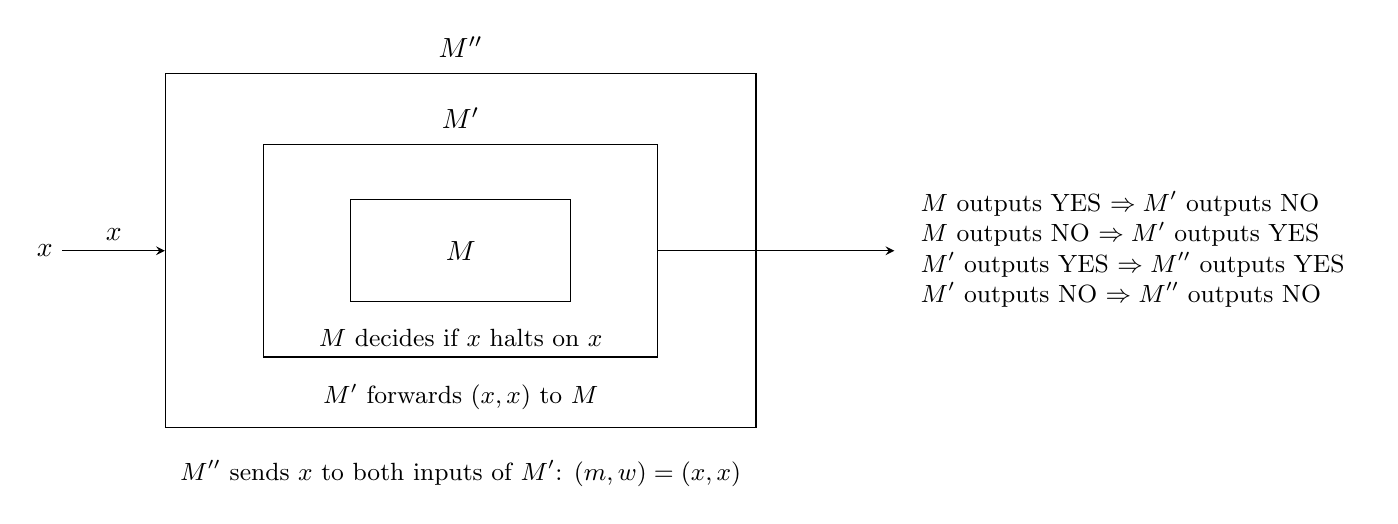
\begin{tikzpicture}[
    box/.style={draw, rectangle, minimum width=7.5cm, minimum height=4.5cm},
    inner/.style={draw, rectangle, minimum width=5cm, minimum height=2.7cm},
    core/.style={draw, rectangle, minimum width=2.8cm, minimum height=1.3cm},
    >=stealth
]

% outer machine
\node[box] (Mpp) {};
\node at (Mpp.north) [above=2pt] {$M''$};

% middle machine
\node[inner] (Mp) at (Mpp.center) {};
\node at (Mp.north) [above=2pt] {$M'$};

% inner machine
\node[core] (M) at (Mp.center) {$M$};

% input arrow
\node[left=1.3cm of Mpp] (input) {$x$};
\draw[->] (input) -- node[above] {$x$} (Mpp.west);

\node[below=8pt of Mpp.south] (step1)
{\small $M''$ sends $x$ to both inputs of $M'$: $(m,w)=(x,x)$};

\node[below=6pt of Mp.south] (step2)
{\small $M'$ forwards $(x,x)$ to $M$};

\node[below=6pt of M.south] (step3)
{\small $M$ decides if $x$ halts on $x$};

% output logic
\node[right=3cm of Mp] (logic)
{\small
\begin{tabular}{l}
$M$ outputs YES $\Rightarrow M'$ outputs NO \\
$M$ outputs NO $\Rightarrow M'$ outputs YES \\
$M'$ outputs YES $\Rightarrow M''$ outputs YES \\
$M'$ outputs NO $\Rightarrow M''$ outputs NO
\end{tabular}
};

\draw[->] (Mp.east) -- (logic.west);

\end{tikzpicture}
\]

Now consider $M''(M'')$. 
\subsubsection*{Case 1: $M''(M'') = NO$}

\end{proof}

\begin{definition}[Recursively Enumerable]
    $L \subseteq \Sigma^*$ is recursively enumerable (RE), if there is a Turing machine $\mathcal{M}$, such that $L = L(\mathcal{M})$. Other equivalent terms for an RE language are: 
    \begin{itemize}
        \item Semi-decidable
        \item Turing recognizable
    \end{itemize}
\end{definition}


\begin{definition}[Recursive]
    $L \subseteq \Sigma^*$ is a recursive(REC) language if there is a Turing machine $\mathcal{M}$, 
    such that $L = L(\mathcal{M})$, and $\mathcal{M}$ is terminating. Recursive languages are also called decidable
\end{definition}

\begin{theorem}
    \[L_H = \{\langle \mathcal{M}, w \rangle \mid w \text{ terminates on } \mathcal M\} \in RE\]
\end{theorem}
\begin{proof}
    We can construct a TM $\mathcal{M}_{Halt}$ which is the turing machine that returns YES if its input machine terminates on input string. 
    \begin{lstlisting}[mathescape=true]
$\mathcal{M}_{Halt}(\mathcal{M}, w)$:
    $\mathcal{M}(w)$
    return YES
    \end{lstlisting}
    This surffice to show that $L_{H} \in RE$
    \subsubsection*{$L_H \notin REC$}
    Similar to how we prove undecidability of the Halting problem
\end{proof}
\begin{theorem}[Membership]
    \[MP = \{\langle \mathcal{M}, w \rangle \mid w \text{ is accepted by } \mathcal{M}\} \in RE\]
\end{theorem}
\begin{proof}
    We can construct TM
    \begin{lstlisting}[mathescape=true]
$\mathcal{M}_{UTM}(\mathcal{M}, w)$:
    $b = \mathcal{M}(w)$
    return $b$
    \end{lstlisting}
\end{proof}

\subsubsection*{Quick Reference: Reduction Recipes}If you are stuck on the construction logic, these are the standard "wrappers" for $M'$:\begin{enumerate}\item \textbf{To show $X$ is "Large" (e.g., Non-Empty):}Construct $M'(x)$ to simulate $M(w)$. If it halts, \textbf{Accept}.\textit{Result:} $L(M')$ is either $\Sigma^*$ (if $M$ halts) or $\emptyset$ (if it loops).\item \textbf{To show $X$ is "Small" (e.g., Empty or Finite):}
To reduce $\overline{L_{Halt}}$ to $L_{Empty}$, use the same construction as above. 
\textit{Logic:} $M$ loops on $w \iff L(M') = \emptyset \iff \langle M' \rangle \in L_{Empty}$.
\begin{table}[h]
\centering
\renewcommand{\arraystretch}{1.5}
\setlength{\tabcolsep}{10pt}
\begin{tabular}{llll}
\textbf{Goal: Show $X$ is...} & \textbf{Hierarchy} & \textbf{Source ($A$)} & \textbf{Requirement} \\ 
Undecidable                   & $\notin \Delta_1$  & $L_{Halt}$            & $A \leq_m X$         \\
Not in RE                     & $\notin \Sigma_1$  & $\overline{L_{Halt}}$ & $A \leq_m X$         \\
Not in co-RE                  & $\notin \Pi_1$     & $L_{Halt}$            & $A \leq_m X$         \\
Not in RE $\cup$ co-RE        & $\notin \Sigma_1 \cup \Pi_1$ & $L_{Total}$ & $A \leq_m X$         \\
\end{tabular}
\caption{Strategic mapping for complexity proofs.}
\end{table}
\item \textbf{To involve all strings (e.g., Totality):}
Construct $M'(x)$ to simulate $M(w)$ for exactly $|x|$ steps. This is often used for more complex $\Pi_2$ proofs.
\end{enumerate}\subsubsection*{The "Direction" Rule}Always remember: Hard $\leq$ New.\begin{itemize}\item You are "borrowing" the difficulty of the known language to prove the unknown one is just as bad.\item If the reduction $f$ maps "Yes" instances to "Yes" instances and "No" to "No", the complexity flows from the source to the target.\end{itemize}
\begin{theorem}
    \[L \in REC \iff \bar{L} \in REC\]
\end{theorem}
\begin{proof}
    $L \in REC \implies \exists \mathcal{M}, L = L(\mathcal{M}), \mathcal{M}$ is terminating, we can construct another TM
    \begin{lstlisting}[mathescape=true]
$\mathcal{M'}(w)$:
    $b = \mathcal{M}(w)$
    return $\neg b$
    \end{lstlisting}
    It is easy to show that $L(\mathcal{M'}) = \bar{L}$, and $\mathcal{M'}$ is terminating.
\end{proof}
\begin{theorem}
    \[L \in RE \land \bar{L} \in RE \implies L \in REC\]
\end{theorem}
\begin{proof}
    Consider then TM for $L$ and $\bar{L}$, $\mathcal{M}_1$ and $\mathcal{M}_2$, we can construct a new TM
    \begin{lstlisting}[mathescape=true]
$\mathcal{M}(w)$:
    for $i > 0$:
        run the $i^{th}$ step of $\mathcal{M}_1$
        if $\mathcal{M}_1$ reaches $q_{\mathcal{M}_1, Acc}$
            return YES
        run the $i^{th}$ step of $\mathcal{M}_2$
        if $\mathcal{M}_2$ reaches $q_{\mathcal{M}_2, Acc}$
            return NO
    \end{lstlisting}
    Since $\forall w, \forall L\subseteq \Sigma^*, w \in L \lor w \in \bar{L}, w$ must be accepted by either $\mathcal{M}_1$ or $\mathcal{M}_2$, 
    therefore $\mathcal{M}$ is terminating.
\end{proof}

\subsection{Reduction}
\begin{definition}
    $L_1 \leq_m L_2$ if there is a computable function $f$, such that 
    \begin{align*}
        w \in L_1 \implies f(w) \in L_2\\
        w \notin L_1 \implies f(w) \notin L_2
    \end{align*}
\end{definition}
\begin{theorem}
    \[L_1 \leq_m L_2, L_2 \in REC \implies L_1 \in REC\]
\end{theorem}
\begin{theorem}
    \[L_1 \leq_m L_2, L_2 \in RE \implies L_1 \in RE\]
\end{theorem}
\begin{proof}
    
\end{proof}
\begin{theorem}
    \[L_1 \leq_m L_2, L_1 \in REC \not\implies L_2 \in REC\]
\end{theorem}
\begin{proof}
    Consider the following recursive language:
    \[L_1 = \{\langle \mathcal{M}, w\rangle \mid w \text{ termintes on } \mathcal{M} \text{ in 10 steps}\}\]
    and 
    \[L_H = \{\langle \mathcal{M}, w\rangle \mid w \text{ termintes on } \mathcal{M}\}\]
    We have shown that $L_H\in RE \setminus REC$. 
    We can construct the following terminating TM to define a computable function $f$
    \begin{lstlisting}[mathescape=true]
$\mathcal{M}_f(\langle \mathcal{M}, w\rangle)$:
    run $\mathcal{M}_1$ on $w$ for 10 steps
    if output is YES:
        return $\langle \mathcal{M}, w\rangle$
    else:
        return $\langle NH, w\rangle$
    \end{lstlisting}
    Where $NH$ is the encoding of a TM that loops forever on all input.\\
    It is easy to show that 
    \[\langle \mathcal{M}, w\rangle \in L_1 \implies f(\langle \mathcal{M}, w\rangle) \in L_H\]
    \[\langle \mathcal{M}, w\rangle \notin L_1 \implies f(\langle \mathcal{M}, w\rangle) \notin L_H\]
    But $L_H \notin REC$ as we have previously shown. Contradiction
\end{proof}


\subsection{RE-hardness}
There are languages beyond the RE class. For example 
\begin{theorem}
    \[\bar{L}_H \notin RE\]
\end{theorem}
\begin{proof}
    Suppose otherwise, $\bar{L}_H \in RE, L_H \in RE \implies L_H \in REC$, contradiction
\end{proof}
\begin{definition}[RE-hard]
    $L$ is RE-hard, if 
    \[\forall L' \in RE, L' \leq_m L\]
\end{definition}
\begin{example}
    \[MP = \{\langle \mathcal{M}, w\rangle \mid w \in L(\mathcal{M})\}\]
    \subsubsection*{$L_{Halt} \leq_m MP$}
    \begin{proof}
        We construct a computable function $f(\langle M, w \rangle) = \langle M', w \rangle$. 
        The machine $M'$ is defined as follows:
        \begin{lstlisting}[mathescape=true]
$M'(x)$:
    Simulate $M$ on input $w$
    Accept // Only reached if $M(w)$ halts
        \end{lstlisting}
        Clearly, $M$ halts on $w \iff M'$ accepts $x$ (for any $x$). 
        Thus $\langle M, w \rangle \in L_{Halt} \iff \langle M', w \rangle \in MP$.
    \end{proof}
\end{example}

Similarly reduction can show some languages are not in RE, if they are at least as hard as a known not in RE language 
\begin{example}
    $\bar{MP} \notin RE$
    \subsubsection*{Proof by Reduction: $\bar{K} \leq_m \bar{MP}$}
    Given $\bar{K} = \{\langle M\rangle \mid \langle M \rangle \notin L(M)\}$ is not in $RE$.
    Define a computable transformation $f(\langle M \rangle) = \langle M', \epsilon \rangle$, where $M'$ is:
    \begin{lstlisting}[mathescape=true]
$M'(x)$:
    Simulate $M$ on input $\langle M \rangle$
    Accept // Only reached if M accepts <M>
    \end{lstlisting}
    \begin{enumerate}
        \item If $\langle M \rangle \in \bar{K}$, then $M$ does not accept $\langle M \rangle$. 
       $M'$ will loop/reject on the simulation, so $L(M') = \emptyset$. 
       Thus, $\epsilon \notin L(M') \implies \langle M', \epsilon \rangle \in \bar{MP}$.
       \item If $\langle M \rangle \notin \bar{K}$, then $M$ accepts $\langle M \rangle$. 
       $M'$ will reach the "Accept" command for any input. 
       Thus, $\epsilon \in L(M') \implies \langle M', \epsilon \rangle \notin \bar{MP}$.
    \end{enumerate}
    
    Conclusion: $\langle M \rangle \in \bar{K} \iff f(\langle M \rangle) \in \bar{MP}$.
\end{example}
\subsection{Validity of FOL}
\begin{definition}
    \[VALID: \{\varphi \mid \varphi \text{ is valid }\}\]
\end{definition}
\begin{theorem}
    $VALID \in RE$
\end{theorem}
\begin{theorem}[Church-Turing Theorem]
    $VALID$ is RE-hard
\end{theorem}







\section{Second Order Logics}
\subsection{Syntax of Second Order Logics}
in second order logics, terms are defined the same as in FOL. 

\[\Sigma = (C, F, R)\]
\[V = FOV \cup SOV\]
where $FOV$ is the set containing variables in FOL, and $SOV$ contains the relation variables, for example
\[SOV = \{X^2, Y^1, ...\}\]
where the superscripts denote the arity of these relation variable. 
\begin{definition}
\[\varphi := t = t \mid R^k(t_1, \dots, t_k) \mid X^k(t_1, \dots, t_k) \mid \neg \varphi \mid \varphi \lor \varphi \mid 
\exists x, \varphi \mid \forall x, \varphi \mid \exists X, \varphi \mid \forall X, \varphi\]    
\end{definition}
\begin{example}
    \[\phi \equiv \forall x, \exists X^1, X(x)\]
    This formula means for all x in the universe, there exist such a unary relation, such that x is in the relation. \\
    This formula is valid as we can always interpret $X = U$.
\end{example}

\subsection*{Semantics of SOL}
Similar to FOL, the semantics of SOL is defined by a structure and an assignment (with free variables)
\[\mathfrak{A} = (U, I)\]
\begin{definition}
    for FOL variable:
    \[\alpha(x) \in U\]
    for SOL variables:
    \[\alpha(X^k) \subseteq U^k\]
    Similar to FOL, model relation is defined recursively:
    \begin{align*}
        &\mathfrak{A}, \alpha \models X^k(t_1, \dots, t_k) &&\iff Val_{\mathfrak{A}, \alpha}(t_1), \dots, Val_{\mathfrak{A}, \alpha}(t_k)) \in \alpha(X)\\
        &\mathfrak{A}, \alpha \models \exists X^k, \phi &&\iff \text{ there is a set of k-ary tuples of } U, S\subseteq U^k\\
        &&&\text{ such that } \mathfrak{A}, \alpha[X \mapsto S] \models \phi\\
        &\mathfrak{A}, \alpha \models \forall X^k, \phi &&\iff \text{ for all sets of k-ary tuples of } U, S\subseteq U^k\\
        &&&\text{ such that } \mathfrak{A}, \alpha[X \mapsto S] \models \phi\\
    \end{align*}
\end{definition}

\subsection{Expressiveness of SOL}
\begin{definition}
    Let $\phi$ be a sentence(no free variables), we can define the set of structures that models $\phi$ as
    \[
    \llbracket \phi \rrbracket = \{\mathfrak{A} \mid \mathfrak{A} \models \phi\}
    \]
\end{definition}
We have proven by compactness of FOL, it is impossible to express the set of all finite/infinite structures with
FOL formula. However we can do so in SOL. 

\subsubsection{Finite structures}
\begin{theorem}
    There exist a SOL formula $\phi_{fin}$ such that
    \[\llbracket \phi_{fin} \rrbracket = \{\mathfrak{A} \mid |U_{\mathfrak{A}}| < \infty\}\]
\end{theorem}
We need to first find some unique property of finite sets
\begin{theorem}
    Let $S$ be a set, $S$ is finite $\iff \forall f: S \mapsto S$ that are injective, $f$ is also surjective 
\end{theorem}

\begin{definition}[structure classes defined by non-sentence]
    For formula $\phi$, where $FVar(\phi) = \{\bar{x}\}$
    \[\llbracket \phi(\bar{x}) \rrbracket = \{(\mathfrak{A}, \bar{e} \in U^k) \mid \mathfrak{A}, \alpha[\bar{x} \mapsto \bar{e}] \models \phi\}\]
\end{definition}

We can first use SOL to define function-like relations. 

\begin{definition}
    A binary relation $S^2 \subseteq U^2$ is function-like, if 
    \begin{enumerate}
        \item $\forall u \in U, \exists v, (u, v) \in S$
        \item $\forall u, v_1, v_2, (u, v_1) \in S \land (u, v_2) \in S \rightarrow (v_1 = v_2)$
    \end{enumerate}
    This is a literal translation of all elements in domain has a value to be mapped to, and no element maps to 2 different elements
\end{definition}

These constraints are be expressed with SOL with free variable: 
\[\phi_{func}(X^2) \equiv \forall x\exists y X(x, y) \land \forall x\forall y \forall z (X(x, y)\land X(x, z) \rightarrow (y = z))\]
\[\phi_{injection}(X^2) \equiv \phi_{func}(X^2) \land \forall x \forall y \forall z(X(x, y) \land X(y, z) \rightarrow (x = y))\]
\[\phi_{surjection}(X^2) \equiv \phi_{func}(X^2) \land \forall y \exists x X(x, y)\]
Therefore, we can use a SOL formula to express finite structures: 
\[\phi_{fin} \equiv \forall X^2 (\phi_{injection}(X^2) \rightarrow \phi_{surjection}(X^2))\]
Follow the same logic as how we proved that it is impossible to express such concept in FOL due to compactness, we can prove that in SOL, compactness does not hold. 

\subsubsection{Reachability}
Consider the following signature: 
\[\Sigma = (\{s, t\}, \emptyset, \{E^2\})\]
\[\mathfrak{C}_{s\leadsto t} = \{\mathfrak{A} \mid I(s) \text{ has a path using } I(E) \text{ to } T(t)\}\]
We have shown this is not expressable in FOL. To express this concept, we need to characterize reachability as a property, which is 
a binary relation that is 
\begin{enumerate}
    \item reflexive
    \item transitive
\end{enumerate}

\[\phi_{reflexive}(X^2) \equiv \forall x X(x, x)\]
\[\phi_{transitive}(X^2) \equiv \forall x\forall y \forall z X(x, y) \land X(y, z) \rightarrow X(x, z)\]

$$\llbracket \phi_{s\leadsto t} \rrbracket \equiv \left\{ (\mathfrak{A} = (U, I), R \subseteq U^2) \mid 
\begin{aligned}
    &\exists w_0, \dots, w_k \in U, \text{ such that:} \\
    &(s, w_0) \in I(E), \\
    &\forall i \in \{0, \dots, k-1\}, (w_i, w_{i+1}) \in I(E), \\
    &(w_k, t) \in I(E)
\end{aligned}
\right\}$$

However we can artificially inflate the set to make it still satisfy the semantics of the formula, but contain more 
pairs that are not connected. We can use the same technique used to define the set of WFF, which is the \textbf{smallest} set.
\begin{definition}
    The set of reachable pairs $\mathfrak{R}$ is the \textbf{smallest} set of pairs that are 
    \begin{enumerate}
        \item $E \subseteq S$
        \item transitive and reflexive
    \end{enumerate}
\end{definition}

First we define the concept of closure
\[\phi_{closed}(X^2) \equiv \phi_{reflexive}(X^2) \land \phi_{transitive}(X^2) \land E \subseteq X \]
the concept of $E$ subsetting $X$ can also be written in SOL as a shorthand
\[\subseteq(X^2) \equiv \forall x\forall y E(x, y) \rightarrow X(x, y)\]
Then we can formally define the relation reachable: 
\[\phi_{reach}(X^2) \equiv \phi_{closed}(X^2) \land \forall Y^2 (\phi_{closed}(Y^2) \rightarrow X^2\supseteq Y^2 )\]


\subsubsection{Cyclic graph}
A cyclic graph is a graph that contains at least one cycle. \\
Irreflaxive reachability can be defined similarly as reachability, but without the reflexive clause. 
\[\phi_{irreflexive\_closed} = \phi_{transitive}(X^2) \land E \subseteq X\]
\[\phi_{irreflexive\_reach}(X^2) \equiv \phi_{irreflexive\_closed} \land \forall Y^2(\phi_{irreflexive\_closed}(Y^2) \rightarrow X^2 \supseteq Y^2)\]
\[\phi_{cyclic} \equiv \exists x \exists X^2(\phi_{irreflexive\_reach}(X^2) \land X(x, x))\]
Alternatively we can use reachability and additional constraints to enforce reflexivity:
\[\exists x \exists y (\exists X^2 \phi_{reach}(X^2) \land E(x, y) \land E(y, x))\]



\subsubsection{Even}
All structures that have finite and even number of elements in the universe
\[\phi_{disjoint}(X_1, X_2) \equiv \forall x X_1(x) \leftrightarrow \neg (X_2(x))\] 
\[\phi_{exhaustive}(X_1, X_2) \equiv \forall x X_1(x) \lor X_2(x)\]
Before we defined a formula to describe relations that are injection-function-like, now we define a formula that describe, there exists a binary relation, between the sets defined by 2 relations.
$$\begin{aligned}
\phi_{injection}(X, Y) \equiv \exists F \Bigl[
& (\forall x : X(x) \rightarrow \exists y : (Y(y) \land F(x, y))) \land \\
& (\forall x, y_1, y_2 : X(x) \land Y(y_1) \land Y(y_2) \land F(x, y_1) \land F(x, y_2) \rightarrow y_1 = y_2) \land \\
& (\forall x_1, x_2, y : X(x_1) \land X(x_2) \land Y(y) \land F(x_1, y) \land F(x_2, y) \rightarrow x_1 = x_2) \Bigr]
\end{aligned}$$
$$\begin{aligned}
\phi_{surjection}(X, Y) \equiv \exists F \Bigl[ 
& (\forall x : X(x) \rightarrow \exists y : (Y(y) \land F(x, y))) \land \\
& (\forall x, y_1, y_2 : X(x) \land Y(y_1) \land Y(y_2) \land F(x, y_1) \land F(x, y_2) \rightarrow y_1 = y_2) \land \\
& (\forall y : Y(y) \rightarrow \exists x : (X(x) \land F(x, y))) \Bigr]
\end{aligned}$$
The first and second lines define totality and function-like property.
\[\phi_{bijection}(X_1, X_2) \equiv \phi_{injection}(X_1, X_2) \land \phi_{surjection}(X_1, X_2)\]
\[\phi_{even} \equiv \exists X^1_1 \exists X^1_2 (\phi_{disjoint}(X_1, X_2) \land \phi_{bijection}(X_1, X_2) \land \phi_{exhaustive}(X_1, X_2))\]


\subsubsection{Bipartite graph}
$$\begin{aligned}
\phi_{bipartite} \equiv \exists X_1^1, X_2^1 \Bigl[ & \phi_{disjoint}(X_1, X_2) \land \phi_{exhaustive}(X_1, X_2) \land \\
& \forall x, y \bigl( E(x, y) \rightarrow \neg(X_1(x) \land X_1(y)) \land \neg(X_2(x) \land X_2(y)) \bigr) \Bigr]
\end{aligned}$$
We can observe that n-partite graphs are exactly thos graphs that are n-colorable, they are identical structures


\subsubsection{Connectedness}A graph is connected if every pair of vertices has a path between them. Since you have already defined $\phi_{reach}(X^2)$, we can use it to define a connected graph.$$\phi_{connected} \equiv \exists X^2 (\phi_{reach}(X^2) \land \forall u \forall v X(u, v))$$Alternatively, we can express it by stating that there is no non-trivial partition of the graph that "cuts" all edges:$$\phi_{connected} \equiv \forall X^1 ((\exists x X(x) \land \exists y \neg X(y)) \rightarrow \exists u \exists v (X(u) \land \neg X(v) \land E(u, v)))$$


\subsubsection{Well-Ordering}In FOL, we can define a total order, but we cannot express that a relation is a well-order (every non-empty set has a least element) because we cannot quantify over sets. In SOL, this is straightforward:Let $\phi_{total}(R^2)$ be the FOL formula for a total order.$$\phi_{well\_order}(R^2) \equiv \phi_{total}(R^2) \land \forall X^1 (\exists x X(x) \rightarrow \exists m (X(m) \land \forall y (X(y) \rightarrow R(m, y))))$$

\subsubsection{Hamiltonian Graphs}A graph is Hamiltonian if it contains a cycle that visits every vertex exactly once. While this property is non-expressible in FOL, it is easily captured in SOL. By Fagin's Theorem, this existential second-order formula ($\Sigma^1_1$) also serves as a proof that the problem is in NP.We define a binary relation $H^2$ to act as a successor relation. The formula $\phi_{hamiltonian}$ is defined as:$$\begin{aligned}
\phi_{hamiltonian} \equiv \exists H^2 \Bigl[ & \underbrace{\phi_{inj}(H^2) \land \phi_{surj}(H^2)}_{\text{Permutation}} \land \underbrace{\forall x\forall y (H(x, y) \rightarrow E(x, y))}_{\text{Sub-graph of } E} \\
& \land \underbrace{\forall X^1 \left( \left( \exists x X(x) \land \forall u\forall v (X(u) \land H(u, v) \rightarrow X(v)) \right) \rightarrow \forall x X(x) \right)}_{\text{Connectivity (Induction Axiom)}} \Bigr]
\end{aligned}$$Logical Breakdown:Permutation: $\phi_{inj} \land \phi_{surj}$ ensures that every vertex has exactly one incoming edge and one outgoing edge in $H$. This forces $H$ to be a collection of one or more disjoint cycles.Sub-graph: Ensures that $H$ only uses edges that actually exist in the original graph $E$.Induction Axiom: This is the "secret sauce." It states that any set $X$ closed under the successor relation $H$ must be the entire universe $U$. This prevents the graph from being split into multiple smaller disjoint cycles (sub-cycles), forcing a single cycle that covers all vertices.
\subsubsection{Well-Foundedness}A relation $E$ is well-founded if there are no infinite descending chains $x_1 \leftarrow x_2 \leftarrow x_3 \dots$. This is equivalent to saying every non-empty set has an $E$-minimal element.$$\phi_{well\_founded} \equiv \forall X^1 (\exists x X(x) \rightarrow \exists m (X(m) \land \forall y (X(y) \rightarrow \neg E(y, m))))$$

\subsubsection{Graph Isomorphism}Another powerful use of SOL is expressing whether two graphs are isomorphic. Given two graphs $\mathfrak{A} = (U_A, E_A)$ and $\mathfrak{B} = (U_B, E_B)$, they are isomorphic if there exists a bijection $f: U_A \to U_B$ that preserves the edge relation.$$\begin{aligned}\phi_{iso} \equiv \exists F^2 \Bigl[&\phi_{bijection}(F^2) \land \\
    & \forall u \forall v \left( E_A(u, v) \leftrightarrow \exists u' \exists v' (F(u, u') \land F(v, v') \land E_B(u', v')) \right) \Bigr]\end{aligned}$$







































































































\end{document}


